%%%%%%%%%%%%%%%%%%%%%%%%%%%%%%%%%%%%%%%%%
% Beamer Presentation
% LaTeX Template
% Version 1.0 (10/11/12)
%
% This template has been downloaded from:
% http://www.LaTeXTemplates.com
%
% License:
% CC BY-NC-SA 3.0 (http://creativecommons.org/licenses/by-nc-sa/3.0/)
%
%%%%%%%%%%%%%%%%%%%%%%%%%%%%%%%%%%%%%%%%%

%----------------------------------------------------------------------------------------
%	PACKAGES AND THEMES
%----------------------------------------------------------------------------------------

\documentclass{beamer}

\mode<presentation> {

% The Beamer class comes with a number of default slide themes
% which change the colors and layouts of slides. Below this is a list
% of all the themes, uncomment each in turn to see what they look like.

%\usetheme{default}
%\usetheme{AnnArbor}
%\usetheme{Antibes}
%\usetheme{Bergen}
%\usetheme{Berkeley}
%\usetheme{Berlin}
%\usetheme{Boadilla}
%\usetheme{CambridgeUS}
%\usetheme{Copenhagen}
\usetheme{Darmstadt}
%\usetheme{Dresden}
%\usetheme{Frankfurt}
%\usetheme{Goettingen}
%\usetheme{Hannover}
%\usetheme{Ilmenau}
%\usetheme{JuanLesPins}
%\usetheme{Luebeck}
%\usetheme{Madrid}
%\usetheme{Malmoe}
%\usetheme{Marburg}
%\usetheme{Montpellier}
%\usetheme{PaloAlto}
%\usetheme{Pittsburgh}
%\usetheme{Rochester}
%\usetheme{Singapore}
%\usetheme{Szeged}
%\usetheme{Warsaw}

% As well as themes, the Beamer class has a number of color themes
% for any slide theme. Uncomment each of these in turn to see how it
% changes the colors of your current slide theme.

%\usecolortheme{albatross}
%\usecolortheme{beaver}
%\usecolortheme{beetle}
%\usecolortheme{crane}
%\usecolortheme{dolphin}
%\usecolortheme{dove}
%\usecolortheme{fly}
\usecolortheme{lily}
%\usecolortheme{orchid}
%\usecolortheme{rose}
%\usecolortheme{seagull}
%\usecolortheme{seahorse}
%\usecolortheme{whale}
%\usecolortheme{wolverine}

%\setbeamertemplate{footline} % To remove the footer line in all slides uncomment this line
%\setbeamertemplate{footline}[page number] % To replace the footer line in all slides with a simple slide count uncomment this line

%\setbeamertemplate{navigation symbols}{} % To remove the navigation symbols from the bottom of all slides uncomment this line
}
\usepackage{tikz}
%\usepackage{ctex}
\usepackage{graphicx} % Allows including images
\usepackage{booktabs} % Allows the use of \toprule, \midrule and \bottomrule in tables
\usetikzlibrary{arrows}

\tikzset{
    left/.style={circle, draw=blue, fill=blue},
    dele/.style={circle, draw=black, fill=black},
    decision/.style={circle, draw=red, fill=red}
}
%----------------------------------------------------------------------------------------
%	TITLE PAGE
%----------------------------------------------------------------------------------------

\title[Joint Equalization]{Joint Equalization and Decoding Scheme using Spinal Codes} % The short title appears at the bottom of every slide, the full title is only on the title page

\author{Yupeng Tai} % Your name
\institute[] % Your institution as it will appear on the bottom of every slide, may be shorthand to save space
{
%State Key Laboratory of Acoustics Institute of Acoustics, Chinese Academy of Sciences\\ % Your institution for the title page
\medskip
\textit{yptai@outlook.com} % Your email address
}
\date{\today} % Date, can be changed to a custom date

\begin{document}

\begin{frame}
\titlepage % Print the title page as the first slide
\end{frame}

\begin{frame}
\frametitle{Overview} % Table of contents slide, comment this block out to remove it
\tableofcontents % Throughout your presentation, if you choose to use \section{} and \subsection{} commands, these will automatically be printed on this slide as an overview of your presentation
\end{frame}

%----------------------------------------------------------------------------------------
%	PRESENTATION SLIDES
%----------------------------------------------------------------------------------------
\section{Introduction of Spinal Code}
\subsection{Encoder}
%***************************************************************
%------------------------------------------------------------------
\begin{frame}
\frametitle{Hash Function}
The Hash Function is a group of function that can be used to map data of arbitrary size to data of fixed size. In the Spinal code we could directly regard it as a \textbf{random number generator} with two inputs: the seed $S(32-bits)$ and message segment $m(k-bits)$; One 32-bits output seed. 
\end{frame}
%-----------------------------------------------------------------
\begin{frame}
\frametitle{Recursive Systematic Convolutional Code}
\begin{columns}
\column{.5\textwidth}
\begin{figure}
\includegraphics[width=.99\textwidth]{Rsccode.pdf}
\end{figure}
\column{.5\textwidth}
We firstly start from this (7,5) RSC code to better understand the Spinal code
\end{columns}
\end{frame}
%-------------------------------------------------
\begin{frame}
\frametitle{Core of Spinal Code}
\begin{columns}
\column{.5\textwidth}
\begin{figure}
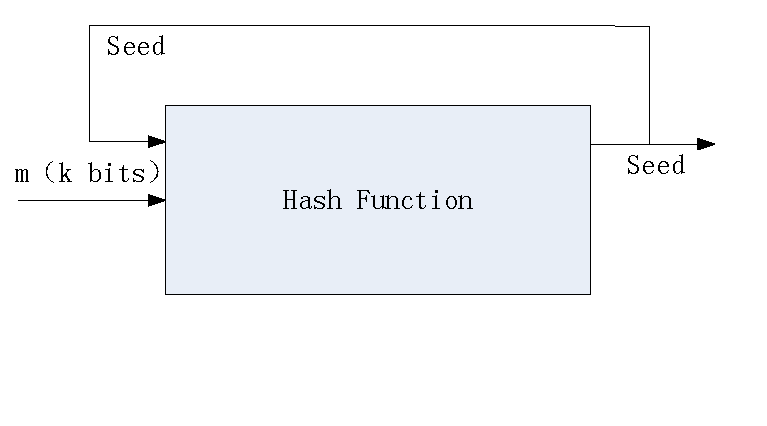
\includegraphics[width=.99\textwidth]{Spinalcode1.pdf}
\end{figure}
\column{.5\textwidth}
There are three modification from the encoder of RSC to the core of Spinal code:
\begin{itemize}
\item  Change the boolean polynomial function into a pseudo-random hash function.
\item Change the input into segments of the message.
\item The feedback and the output is a 32-bit seed.
\item Don't transmit the message itself (not a system code).
\end{itemize}
\end{columns}
\end{frame}
%-------------------------------------------------
\begin{frame}
\frametitle{Converse the recursive structure into sequence structure}
\begin{figure}
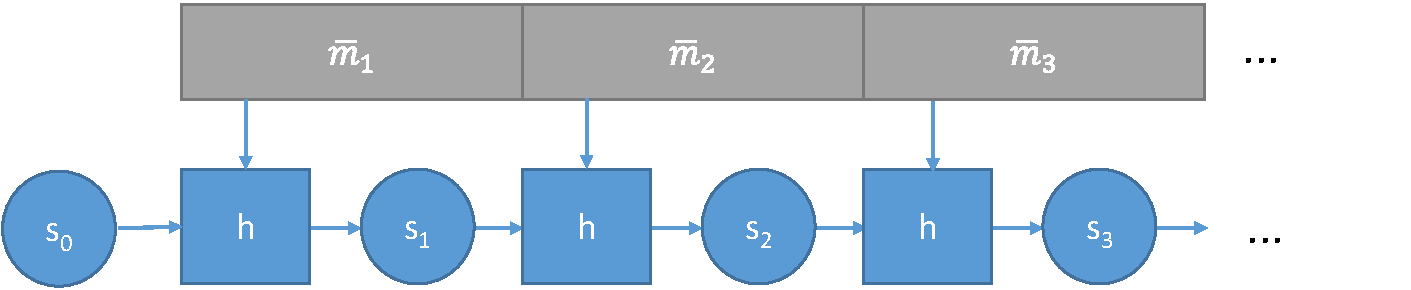
\includegraphics[width=.99\textwidth]{Spinalcode2.pdf}
\end{figure}
The message length is n, $\overline{m}_i$ is the k-bits segment of message. h represent the hash function. $s_i$ is the seeds. 
\end{frame}
%-------------------------------------------------
\begin{frame}
\frametitle{The whole encode scheme}
%To generate the code for transmission. Add random number generators (GNR) which are seeded by each seeds.
\begin{columns}
\column{.6\textwidth}
\begin{figure}
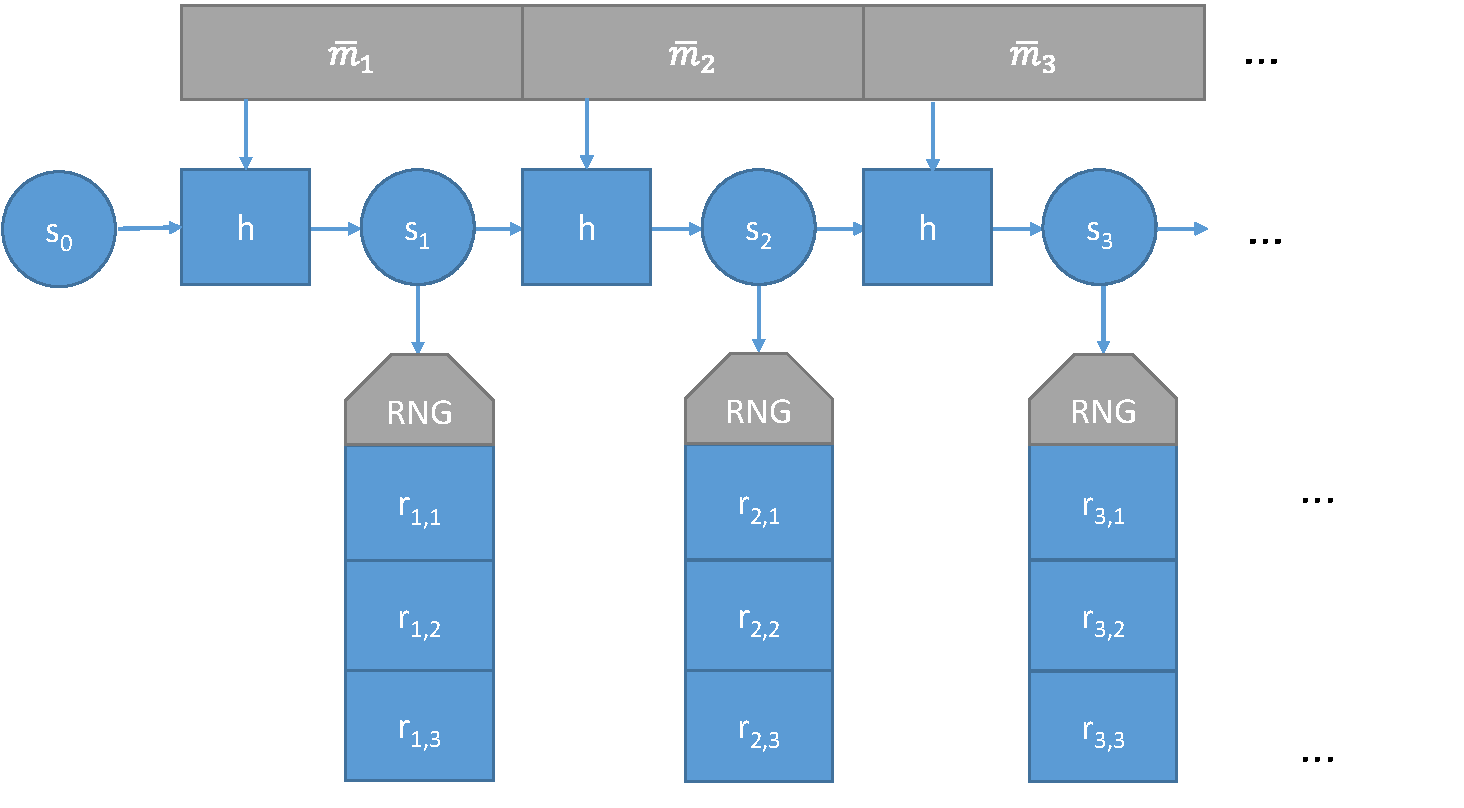
\includegraphics[width=.99\textwidth]{Spinalcode3.pdf}
\end{figure}
\column{.4\textwidth}
\begin{itemize}
\item $r_{i,j}$ is the $j^{th}$ output of GNR seed by $s_i$. In fact the primal output generated by GNR is 32-bit. The final output is the lowest $c$-bits of primal ones.

\item The size of $c$ is depended on the mapper's degree. So the range of $c$ is (1,32). Increasing the $c$ would not increase the encoding complexity.
\end{itemize}
\end{columns}
\end{frame}
%-------------------------------------------------
\begin{frame}
\frametitle{Rateless transmission scheme}
\begin{figure}
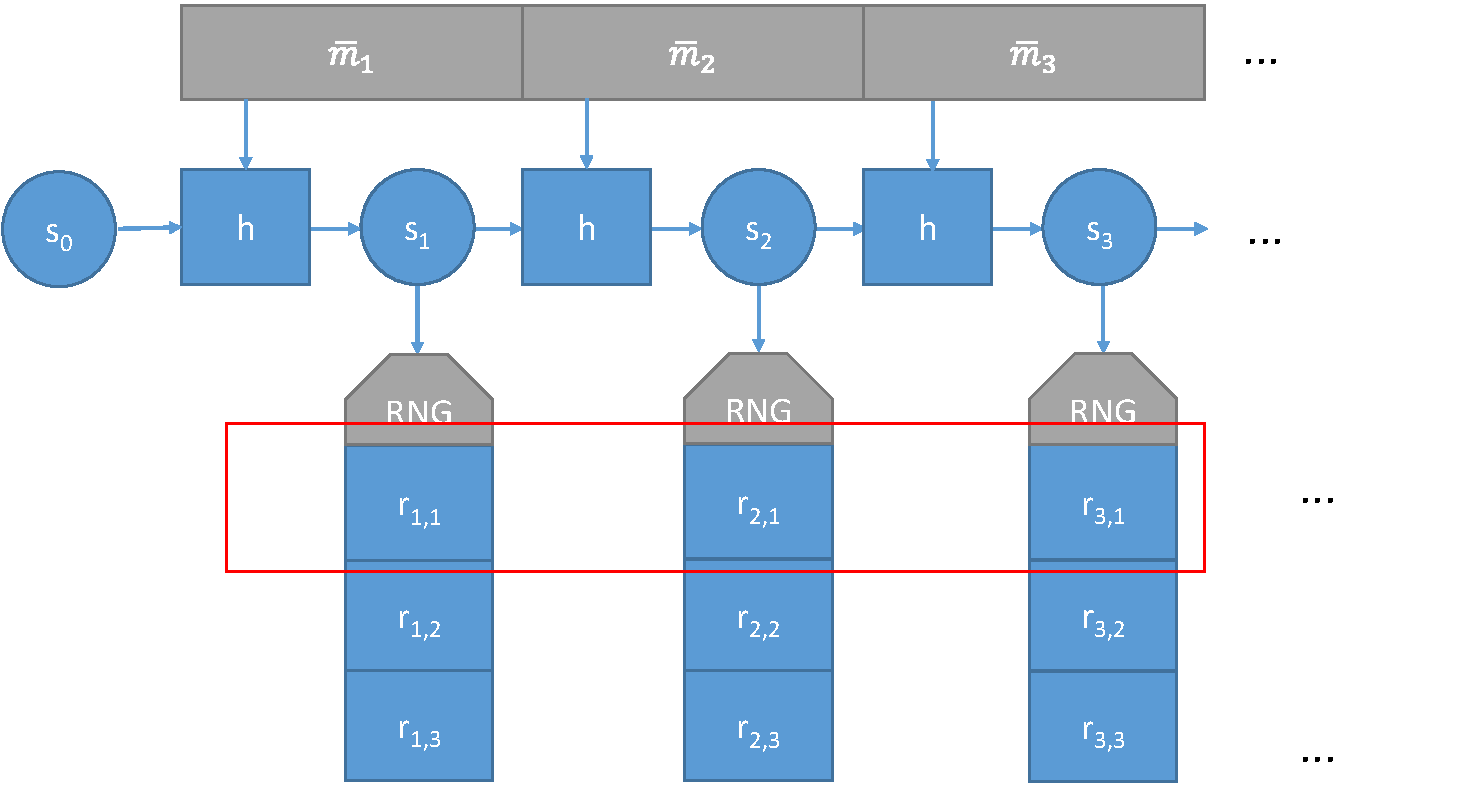
\includegraphics[width=.99\textwidth]{Spinalcode4.pdf}
\end{figure}
\end{frame}
%-------------------------------------------------
\begin{frame}
\frametitle{Rateless transmission scheme}
\begin{figure}
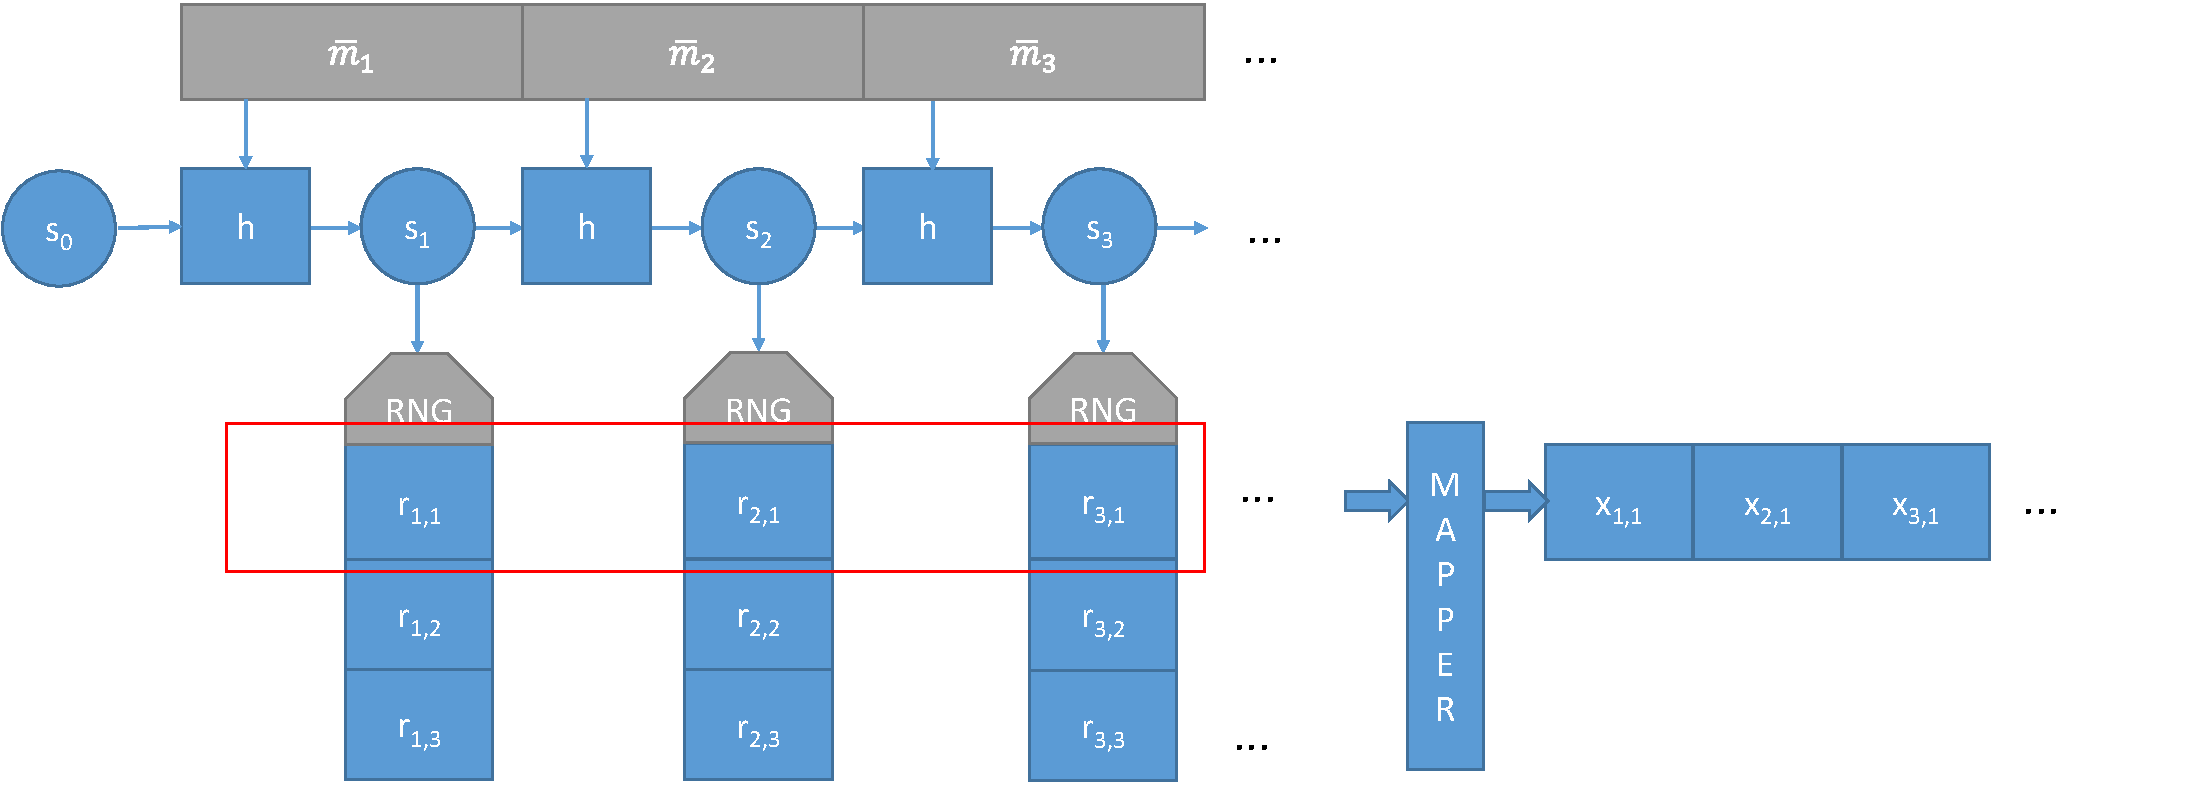
\includegraphics[width=.99\textwidth]{Spinalcode5.pdf}
\end{figure}
\end{frame}
%-------------------------------------------------
\begin{frame}
\frametitle{Rateless transmission scheme}
\begin{figure}
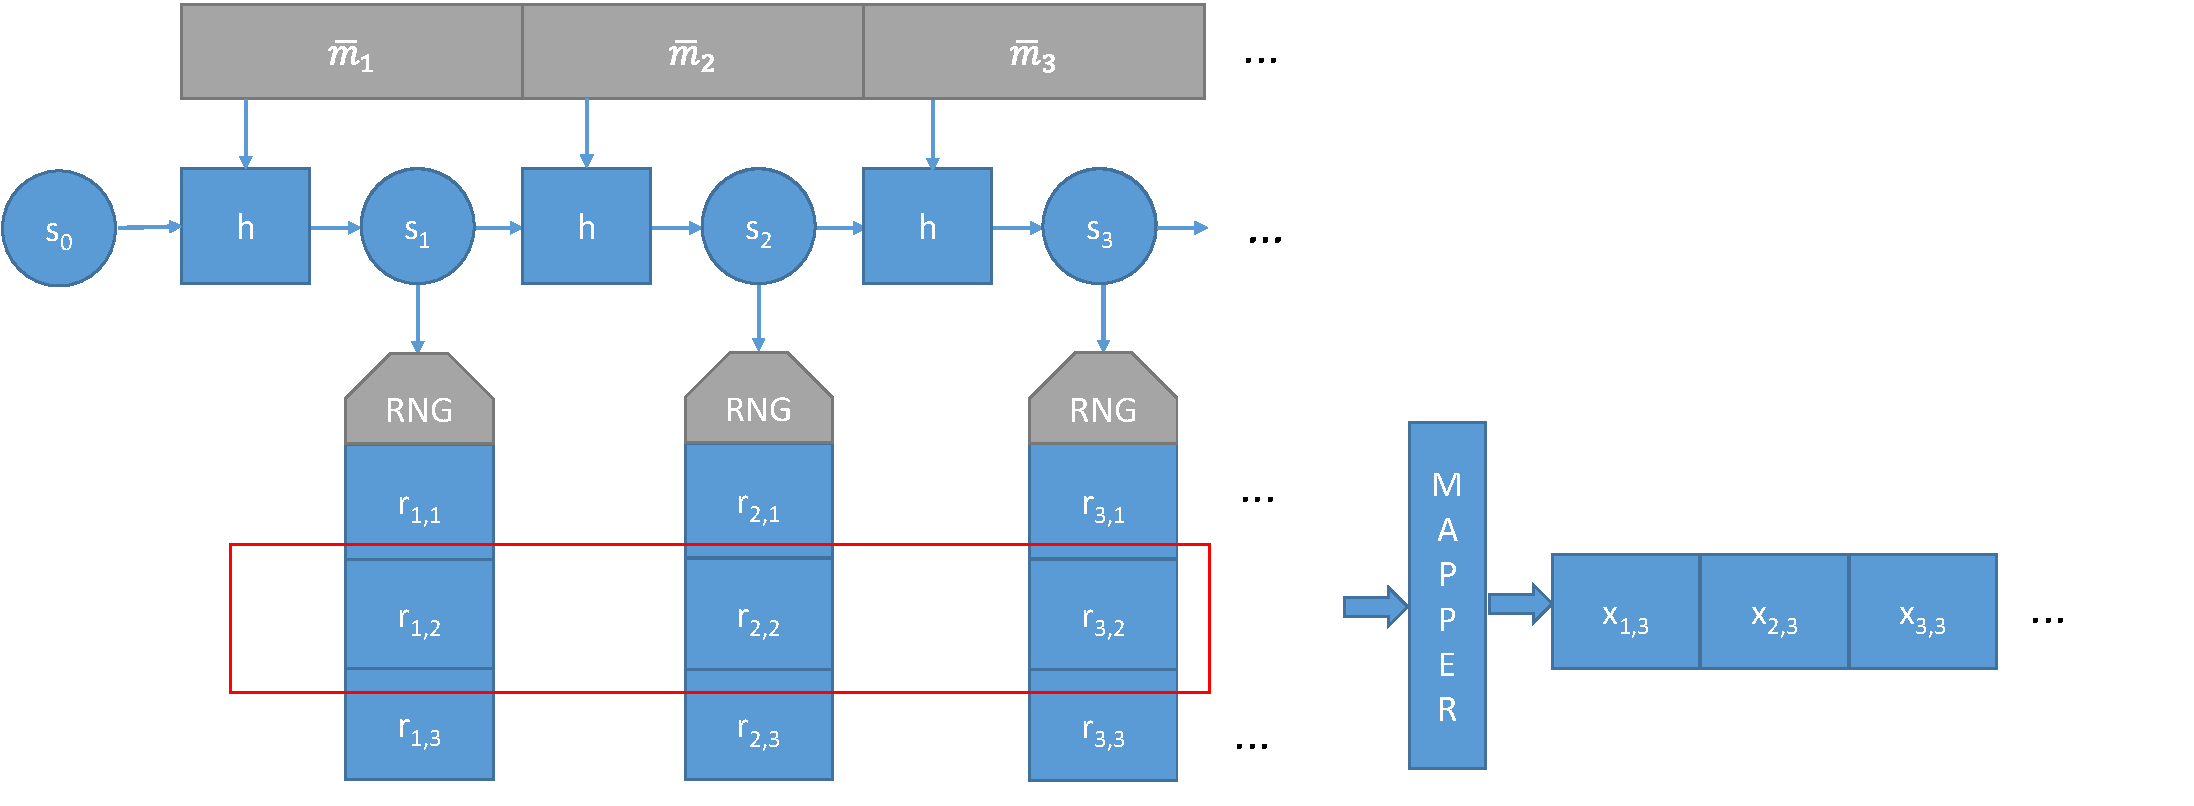
\includegraphics[width=.99\textwidth]{Spinalcode6.pdf}
\end{figure}
\end{frame}
%-------------------------------------------------
\begin{frame}
\frametitle{Rateless transmission scheme}
\begin{figure}
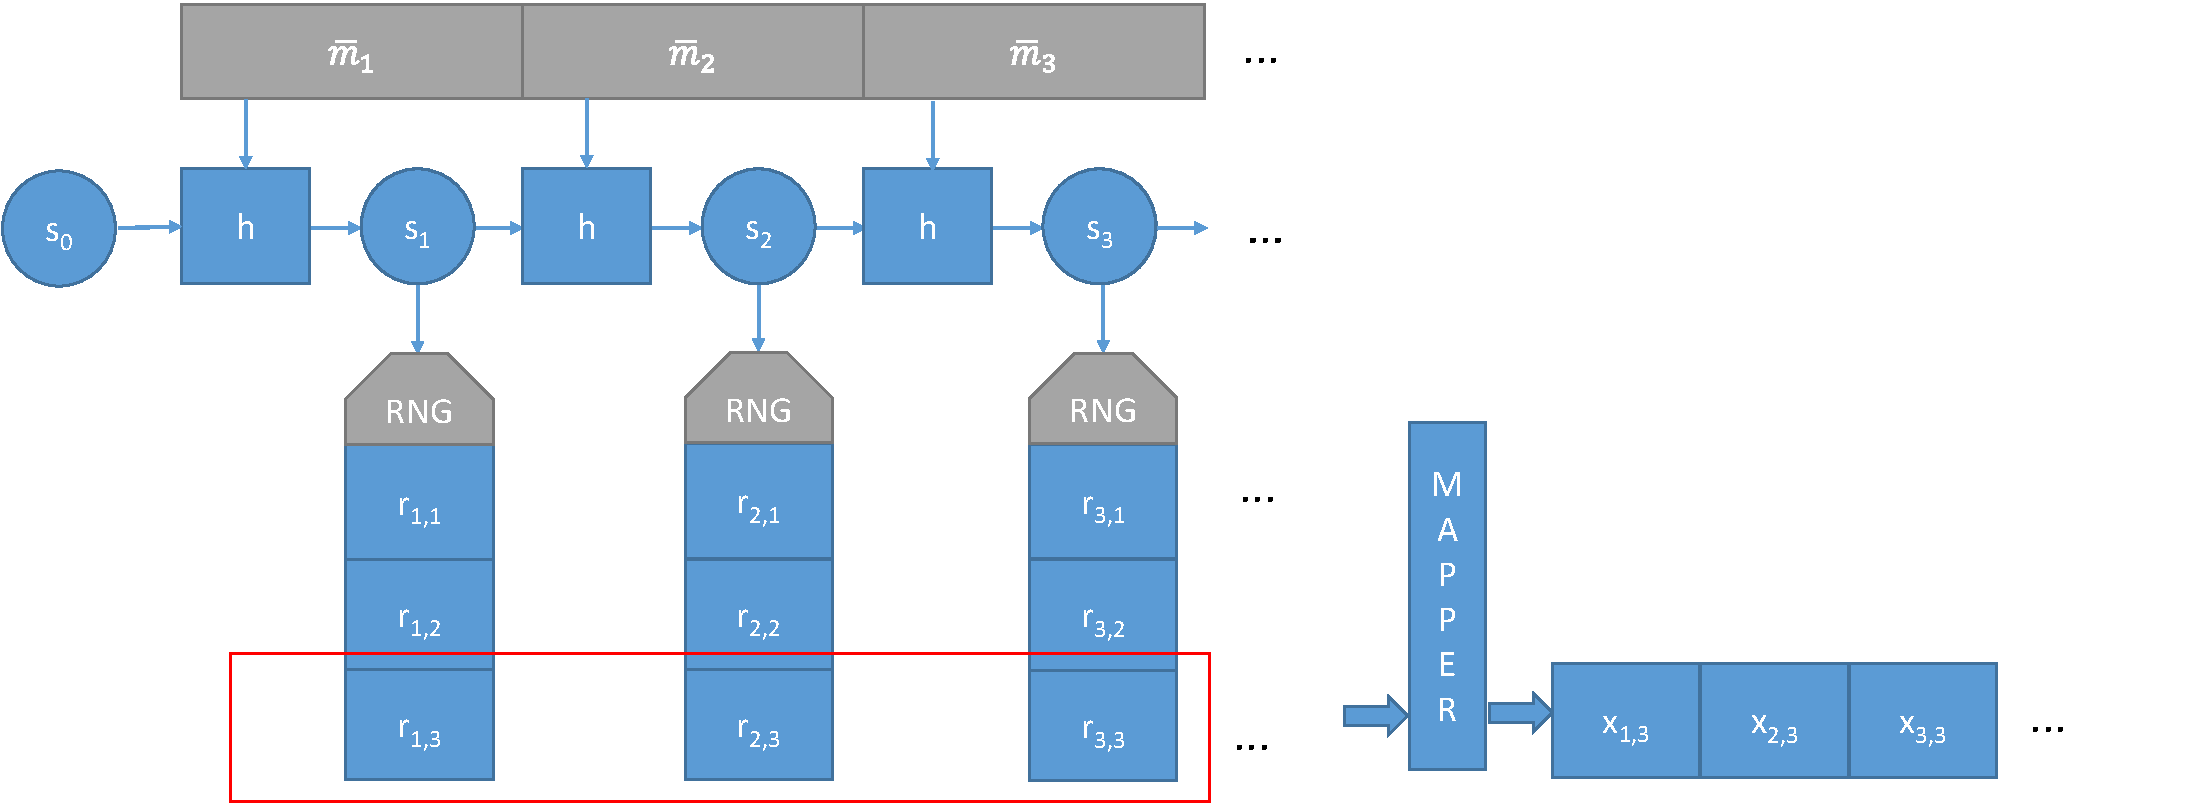
\includegraphics[width=.99\textwidth]{Spinalcode7.pdf}
\end{figure}
\end{frame}
%-------------------------------------------------
%*************************************************
\subsection{Decoder}
%*************************************************
%-------------------------------------------------

%-------------------------------------------------
\begin{frame}
\frametitle{ML decoder}
{\small As the hash function could not be reverse. So the decode method is replay the encoder. A simply example: the k=1, transmitted message is '1' '0'.}
\begin{figure}
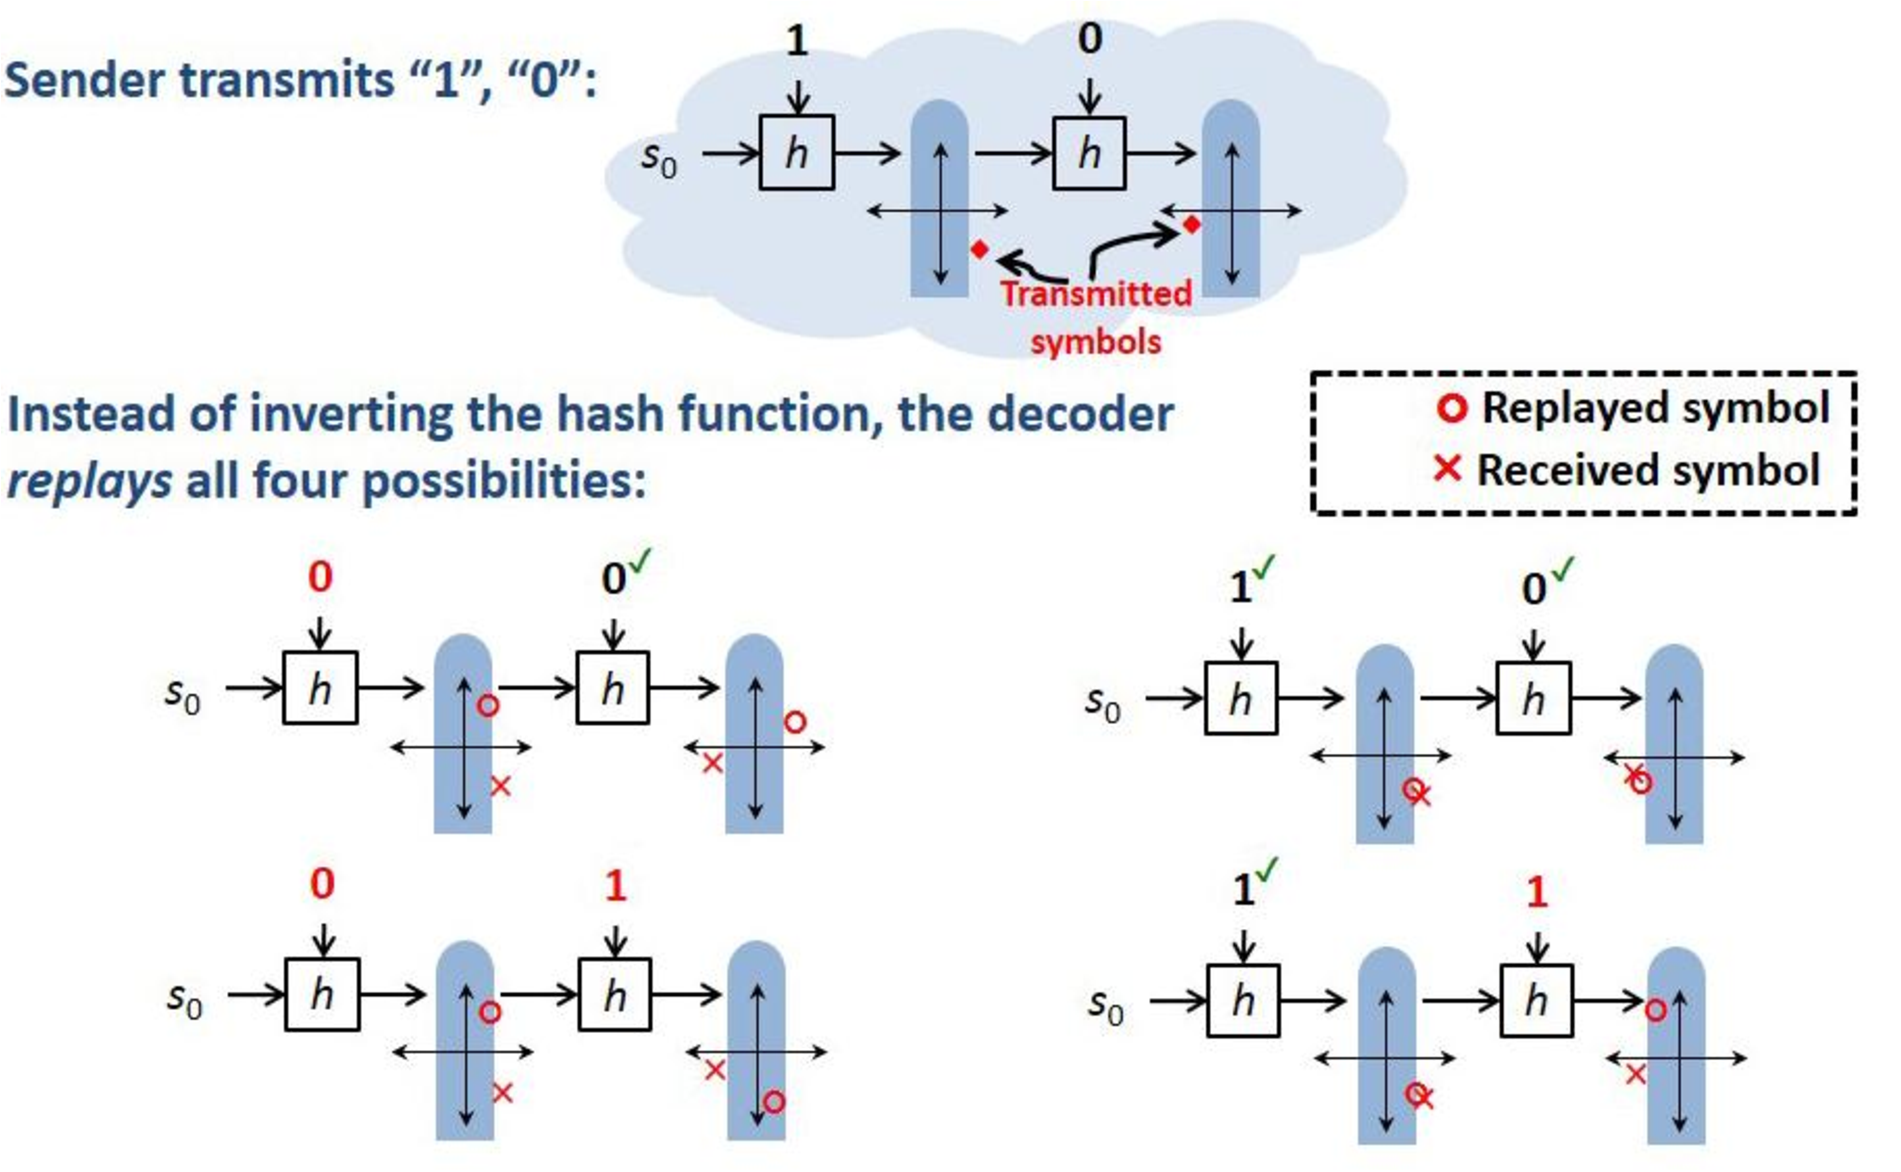
\includegraphics[width=.8\textwidth]{Spinaldecode1.pdf}
\end{figure}
\end{frame}
%-------------------------------------------------
\begin{frame}
\frametitle{ML decoder}
Measure total distance.
\begin{figure}
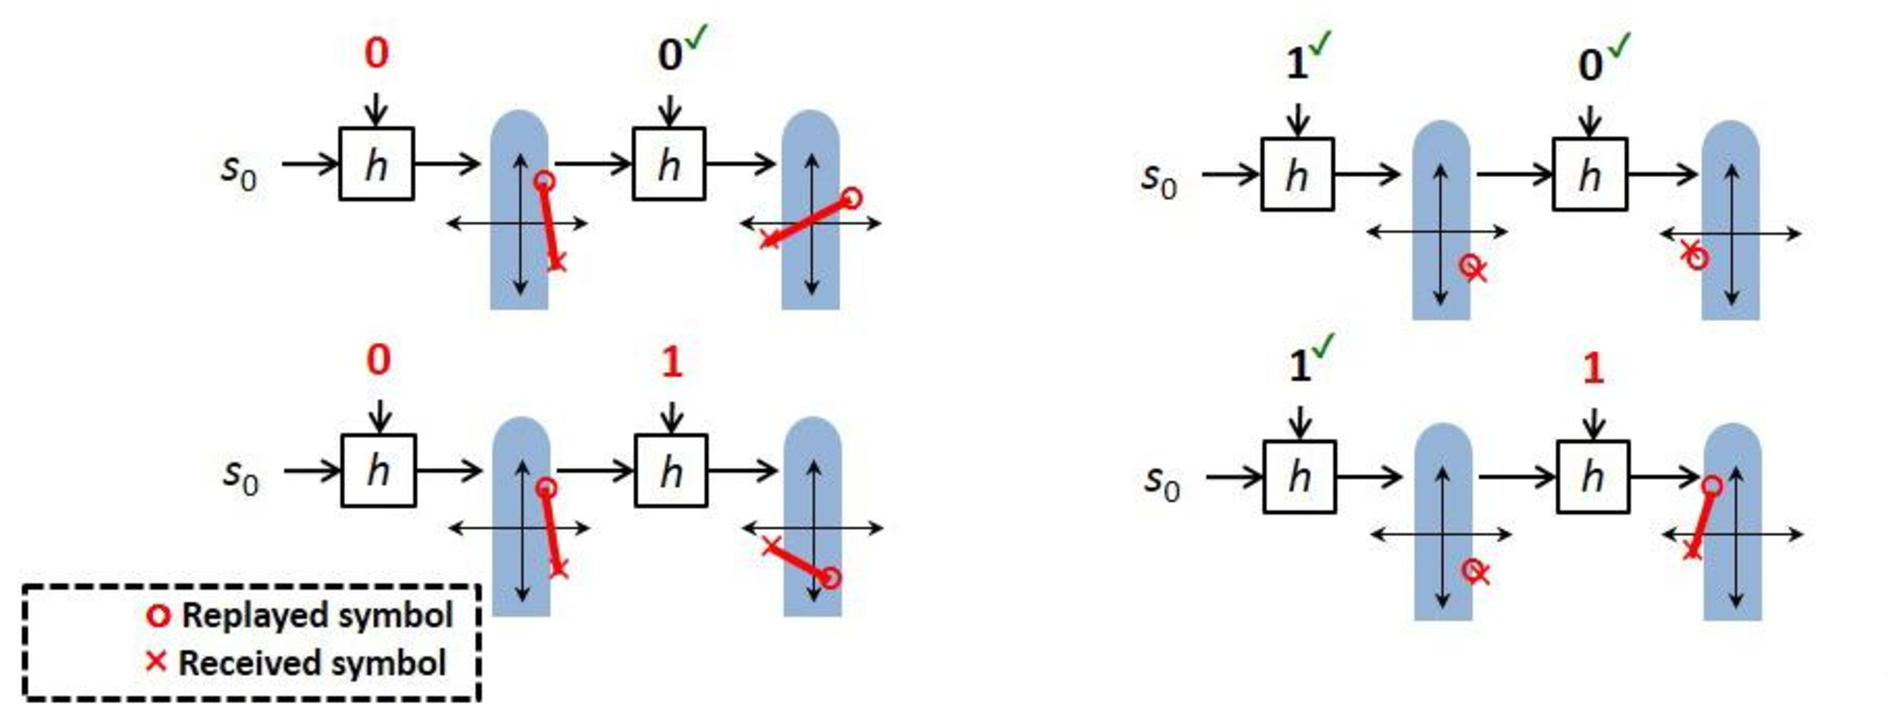
\includegraphics[width=.99\textwidth]{Spinaldecode2.pdf}
\end{figure}
\end{frame}
%-------------------------------------------------
\begin{frame}
\frametitle{Tree decoder algorithm}
\begin{figure}
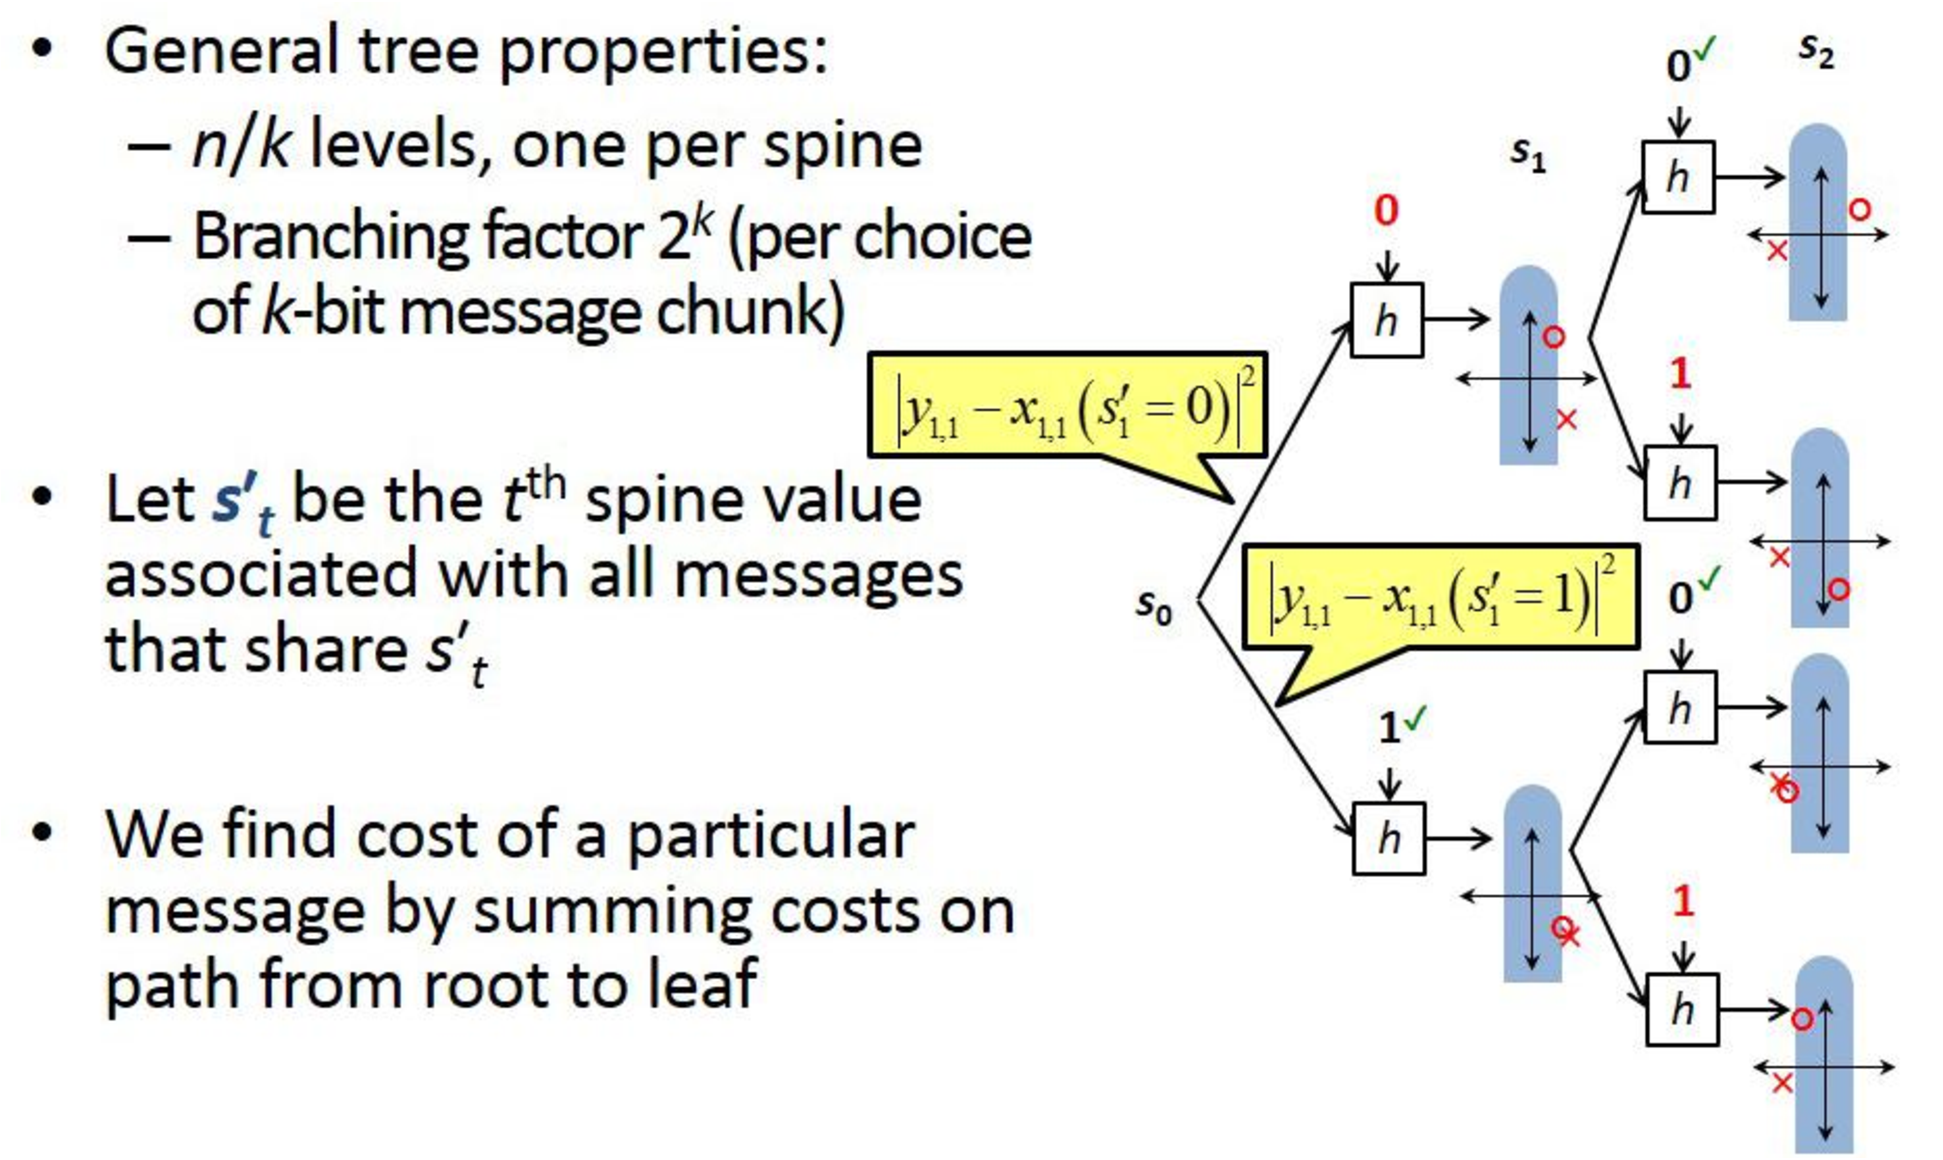
\includegraphics[width=.99\textwidth]{Spinaldecode3.pdf}
\end{figure}
\end{frame}
%--------------------------------------------------
\begin{frame}
\frametitle{Tree decoder algorithm}
\begin{figure}
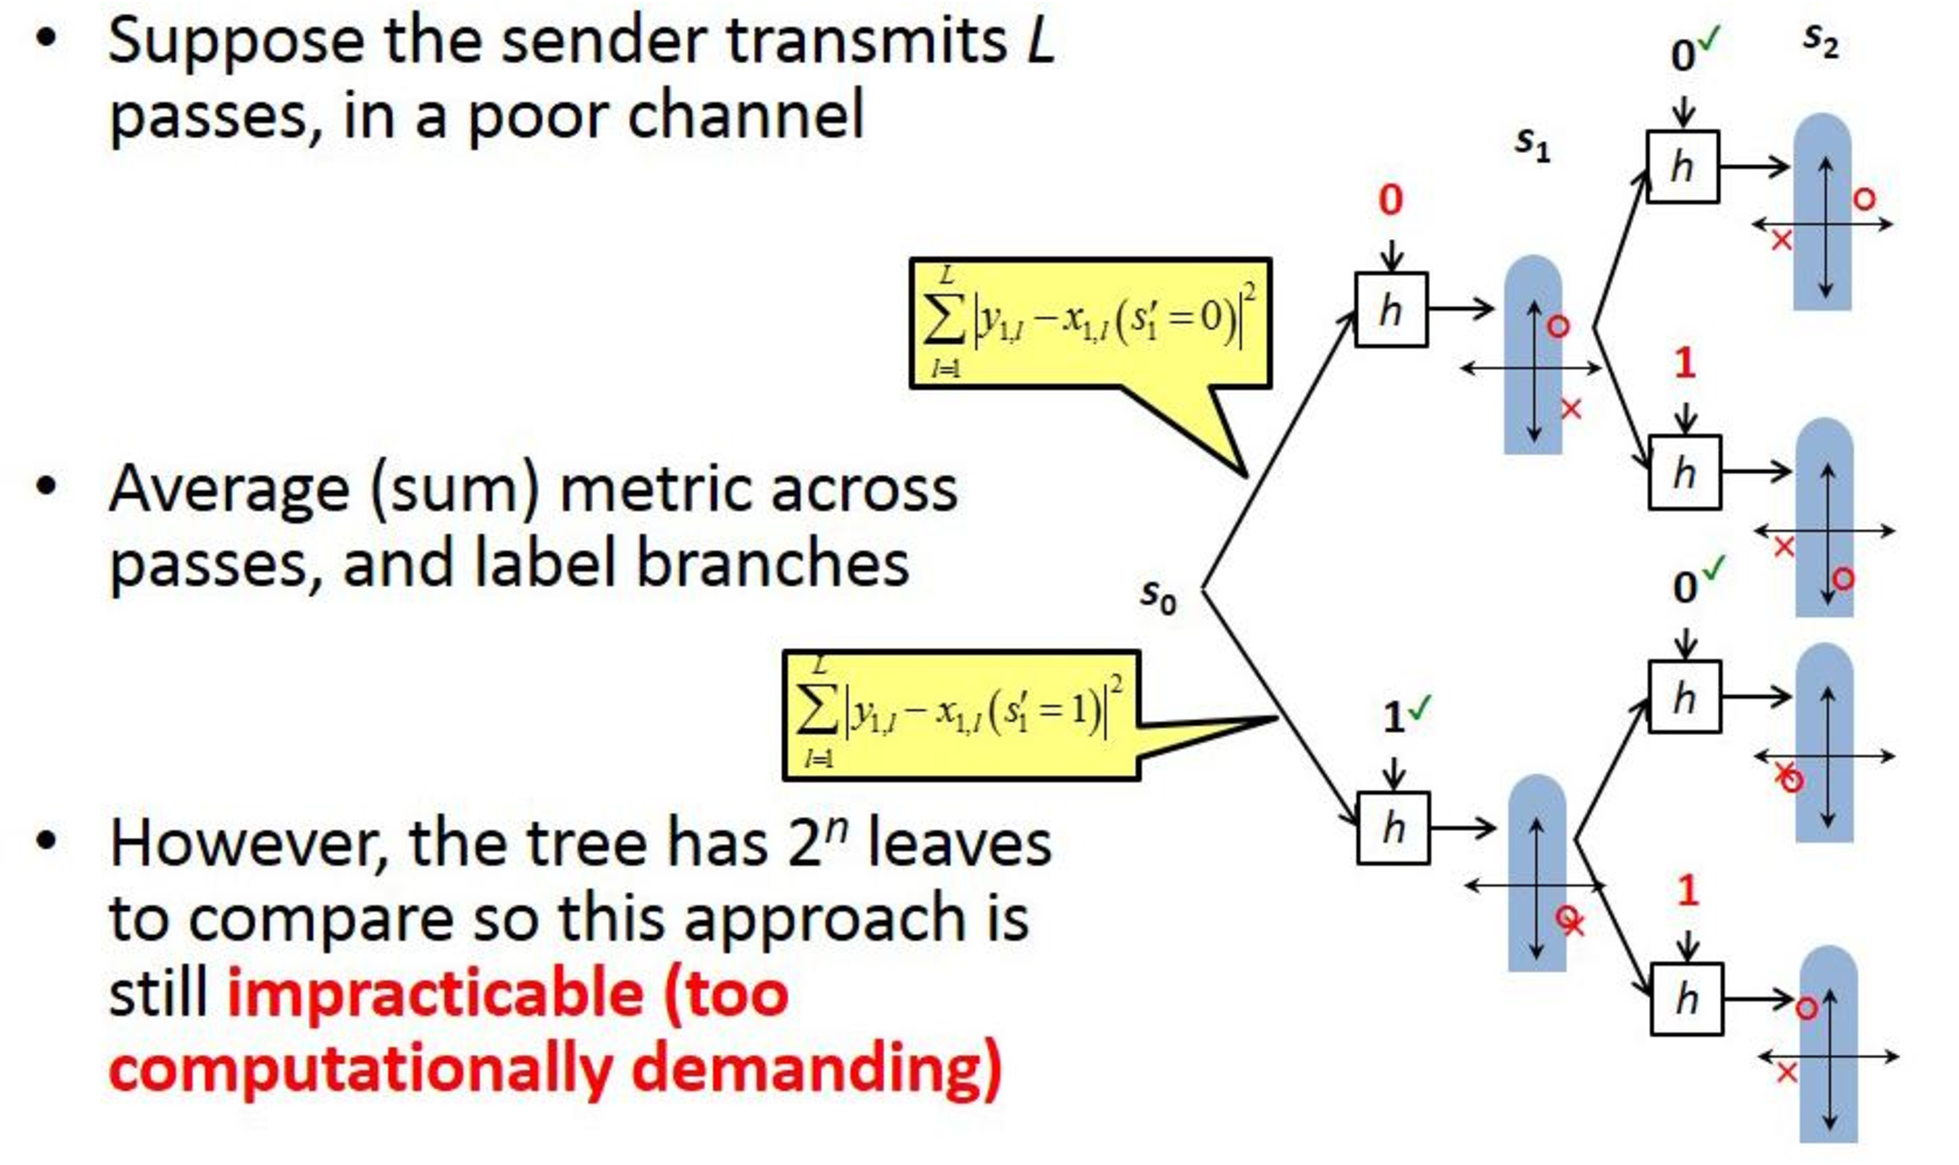
\includegraphics[width=.99\textwidth]{Spinaldecode4.pdf}
\end{figure}
\end{frame}
%---------------------------------------------------
\begin{frame}
\frametitle{Approximate ML decoder: k=1,B=2 -- Initialization}

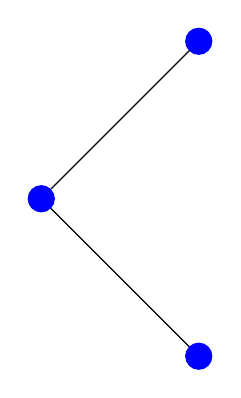
\begin{tikzpicture}
  [
    grow                    = right,
    sibling distance        = 4cm,
    level distance          = 2cm,
    every node/.style       = {font=\footnotesize},
  ]
  \node [left] {}
    child {[sibling distance=2cm] node [left] {}}
    child {[sibling distance=2cm] node [left] {}}
    ;
\end{tikzpicture}
\end{frame}
%--------------------------------------------------
\begin{frame}
\frametitle{Approximate ML decoder: k=1,B=2 -- Expand}

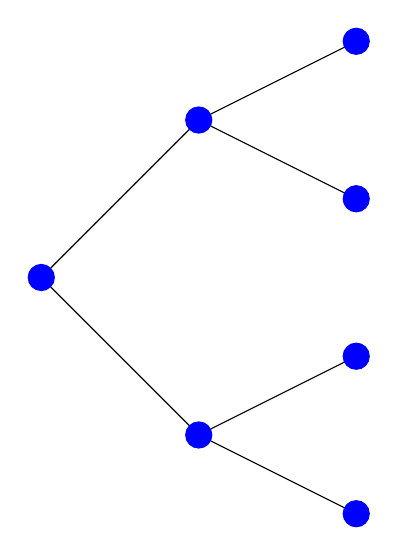
\begin{tikzpicture}
  [
    grow                    = right,
    sibling distance        = 4cm,
    level distance          = 2cm,
    every node/.style       = {font=\footnotesize},
  ]
  \node [left] {}
    child { [sibling distance=2cm] node [left] {}
    	child { [sibling distance=1.2cm] node [left] {}}
    	child { [sibling distance=1.2cm]node [left] {}}
    	}
    child {[sibling distance=2cm] node [left] {}
        child {[sibling distance=1.2cm] node [left] {}}
    	child { [sibling distance=1.2cm]node [left] {}}
    	}
    ;
\end{tikzpicture}
\end{frame}
%--------------------------------------------------
%--------------------------------------------------
\begin{frame}
\frametitle{Approximate ML decoder: k=1,B=2 -- Score and Prune}

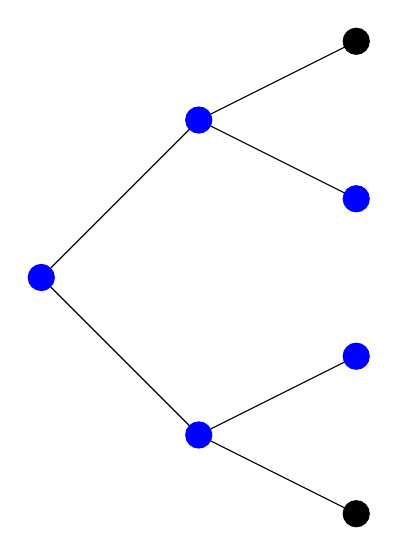
\begin{tikzpicture}
  [
    grow                    = right,
    sibling distance        = 4cm,
    level distance          = 2cm,
    every node/.style       = {font=\footnotesize},
  ]
  \node [left] {}
    child { [sibling distance=2cm] node [left] {}
    	child { [sibling distance=1.2cm] node [dele] {}}
    	child { [sibling distance=1.2cm]node [left] {}}
    	}
    child {[sibling distance=2cm] node [left] {}
        child {[sibling distance=1.2cm] node [left] {}}
    	child { [sibling distance=1.2cm]node [dele] {}}
    	}
    ;
\end{tikzpicture}
\end{frame}
%--------------------------------------------------
\begin{frame}
\frametitle{Approximate ML decoder: k=1,B=2 -- Expand}

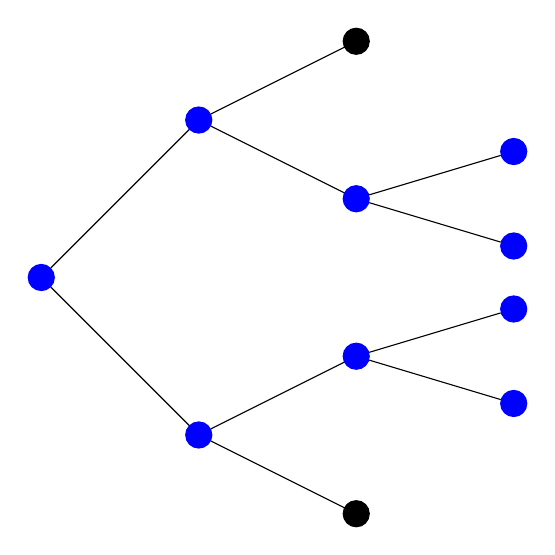
\begin{tikzpicture}
  [
    grow                    = right,
    sibling distance        = 4cm,
    level distance          = 2cm,
    every node/.style       = {font=\footnotesize},
  ]
  \node [left] {}
    child { [sibling distance=2cm] node [left] {}
    	child { [sibling distance=1.2cm] node [dele] {}}
    	child { [sibling distance=1.2cm]node [left] {}
    	    child{node[left] {}}
    		child{node[left] {}}}}
    child {[sibling distance=2cm] node [left] {}
        child {[sibling distance=1.2cm] node [left] {}
            child{node[left] {}}
    		child{node[left] {}} }
    	child { [sibling distance=1.2cm]node [dele] {}}}
    ;
\end{tikzpicture}
\end{frame}
%--------------------------------------------------
\begin{frame}
\frametitle{Approximate ML decoder: k=1,B=2 -- Score and Prune}

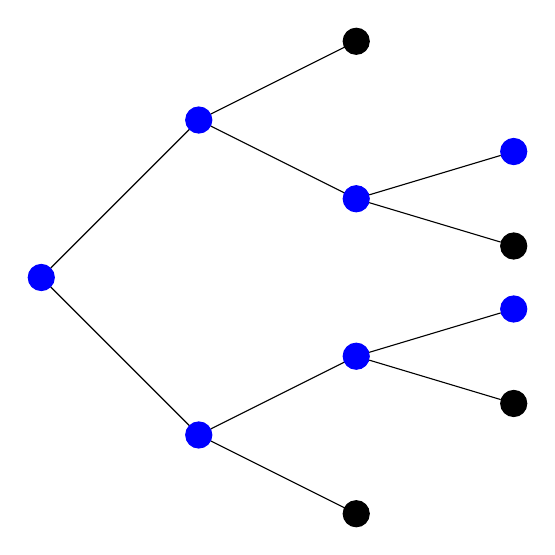
\begin{tikzpicture}
  [
    grow                    = right,
    sibling distance        = 4cm,
    level distance          = 2cm,
    every node/.style       = {font=\footnotesize},
  ]
  \node [left] {}
    child { [sibling distance=2cm] node [left] {}
    	child { [sibling distance=1.2cm] node [dele] {}}
    	child { [sibling distance=1.2cm]node [left] {}
    	    child{node[dele] {}}
    		child{node[left] {}}}}
    child {[sibling distance=2cm] node [left] {}
        child {[sibling distance=1.2cm] node [left] {}
            child{node[dele] {}}
    		child{node[left] {}} }
    	child { [sibling distance=1.2cm]node [dele] {}}}
    ;
\end{tikzpicture}
\end{frame}
%--------------------------------------------------
\begin{frame}
\frametitle{Approximate ML decoder: k=1,B=2 -- Expand}

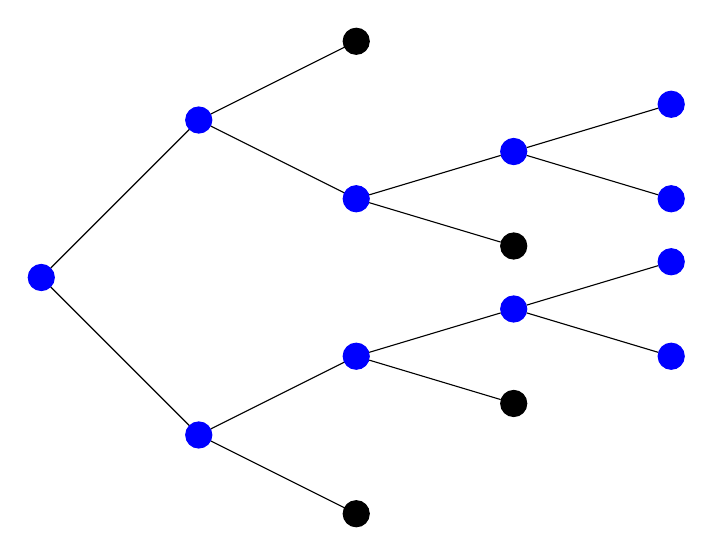
\begin{tikzpicture}
  [
    grow                    = right,
    sibling distance        = 4cm,
    level distance          = 2cm,
    every node/.style       = {font=\footnotesize},
  ]
  \node [left] {}
    child { [sibling distance=2cm] node [left] {}
    	child { [sibling distance=1.2cm] node [dele] {}}
    	child { [sibling distance=1.2cm]node [left] {}
    	    child{node[dele] {}}
    		child{node[left] {}
    		    child{node[left]{}}
    			child{node[left]{}}}}}
    child {[sibling distance=2cm] node [left] {}
        child {[sibling distance=1.2cm] node [left] {}
            child{node[dele] {}}
    		child{node[left] {}
    			child{node[left]{}}
    			child{node[left]{}}}}
    	child { [sibling distance=1.2cm]node [dele] {}}}
    ;
\end{tikzpicture}
\end{frame}
%--------------------------------------------------
\begin{frame}
\frametitle{Approximate ML decoder: k=1,B=2 -- Make Decision}

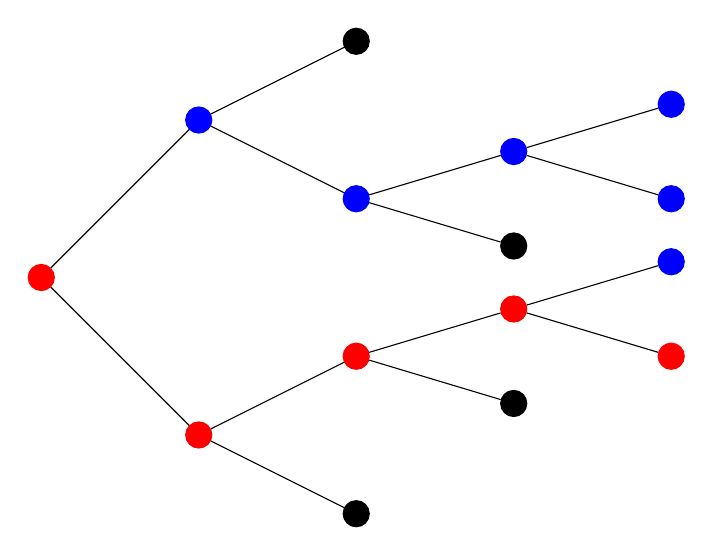
\begin{tikzpicture}
  [
    grow                    = right,
    sibling distance        = 4cm,
    level distance          = 2cm,
    every node/.style       = {font=\footnotesize},
  ]
  \node [decision] {}
    child { [sibling distance=2cm] node [decision] {}
    	child { [sibling distance=1.2cm] node [dele] {}}
    	child { [sibling distance=1.2cm]node [decision] {}
    	    child{node[dele] {}}
    		child{node[decision] {}
    		    child{node[decision]{}}
    			child{node[left]{}}}}}
    child {[sibling distance=2cm] node [left] {}
        child {[sibling distance=1.2cm] node [left] {}
            child{node[dele] {}}
    		child{node[left] {}
    			child{node[left]{}}
    			child{node[left]{}}}}
    	child { [sibling distance=1.2cm]node [dele] {}}}
    ;
\end{tikzpicture}
\end{frame}
%--------------------------------------------------
\section{My Simulation and Results} % Sections can be created in order to organize your presentation into discrete blocks, all sections and subsections are automatically printed in the table of contents as an overview of the talk
%------------------------------------------------
\begin{frame}
\frametitle{The results of ML decoder and approximate ML decoder}
\begin{columns}
\column{.5\textwidth}
\begin{figure}
\includegraphics[width=.99\textwidth]{Rsccode.pdf}
\end{figure}
\column{.5\textwidth}
We firstly start from this (7,5) RSC code to better understand the Spinal code
\end{columns}
\end{frame}

\subsection{Modification of Pass Transition Method } % A subsection can be created just before a set of slides with a common theme to further break down your presentation into chunks

%------------------------------------------

\begin{frame}
\frametitle{ML equalization}
\begin{itemize}
\item A frequency-selective channel: $y_n=\sum_{l=0}^Lh_lx_{n-l}+w_n$
\item The ML equalization rule: 
$\widehat{M} =arg \min\limits_{m_i\in\{0\cdots2^q\}}(\sum_{i=1}^n\Vert y_i-\sum_{l=1}^Lh_lx_{i-l}(m_{i-l})\Vert )$
\item Considering the encoding process where $m_(i-l)$ are generated by RNG with seed $s_j$ so 
 $\widehat{M} =arg \min\limits_{m_i\in\{0\cdots2^q\}}(\sum_{i=1}^n\Vert y_i-\sum_{l=1}^Lh_lx_{i-l}(RNG(s_j))\Vert )$
\end{itemize}
\end{frame}
%----------------------------------------------------------

\begin{frame}
\frametitle{Simulation Results 1}
\begin{columns}[c]
\column{.7\textwidth}
\begin{figure}
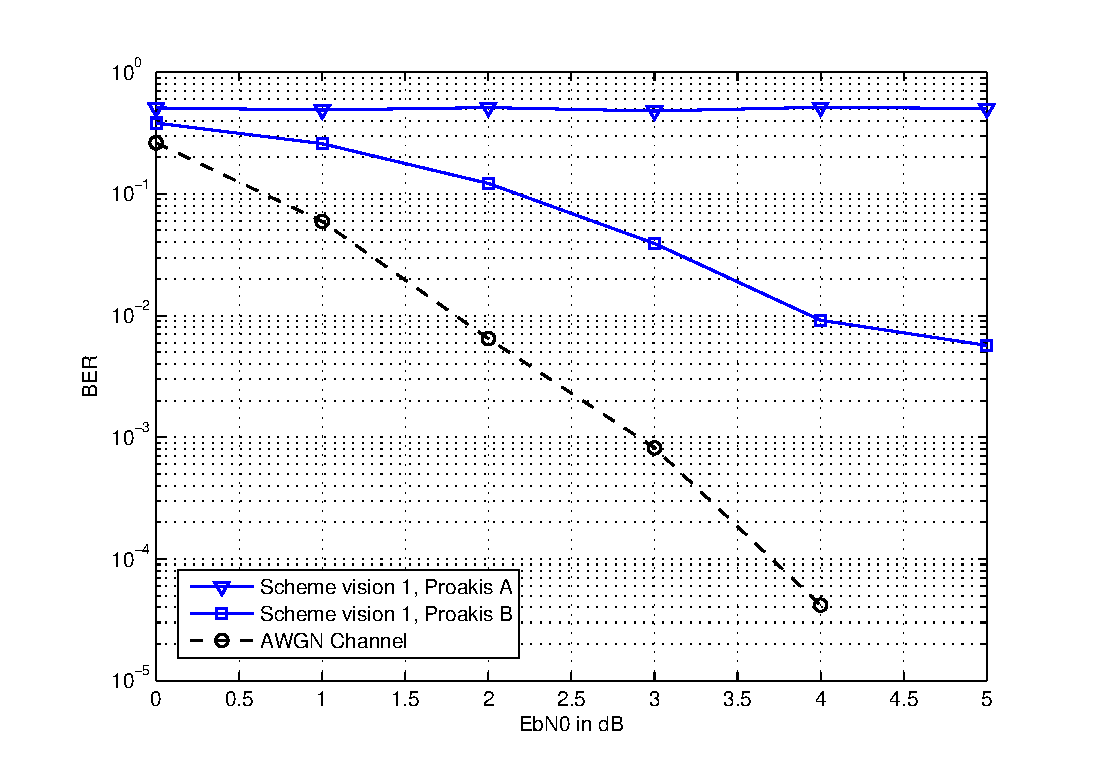
\includegraphics[width=.99\textwidth]{figure_vision1.eps}%wait for figure
\end{figure}
\column{.3\textwidth}
The results didn't desirable. 

The mainly reason is the correlations between the spines are too strong and make the beam algorithm prune the wrong branch.
\end{columns}

\end{frame}

%----------------------------------------------------------
\begin{frame}
\frametitle{Original Diagram}
\begin{figure}
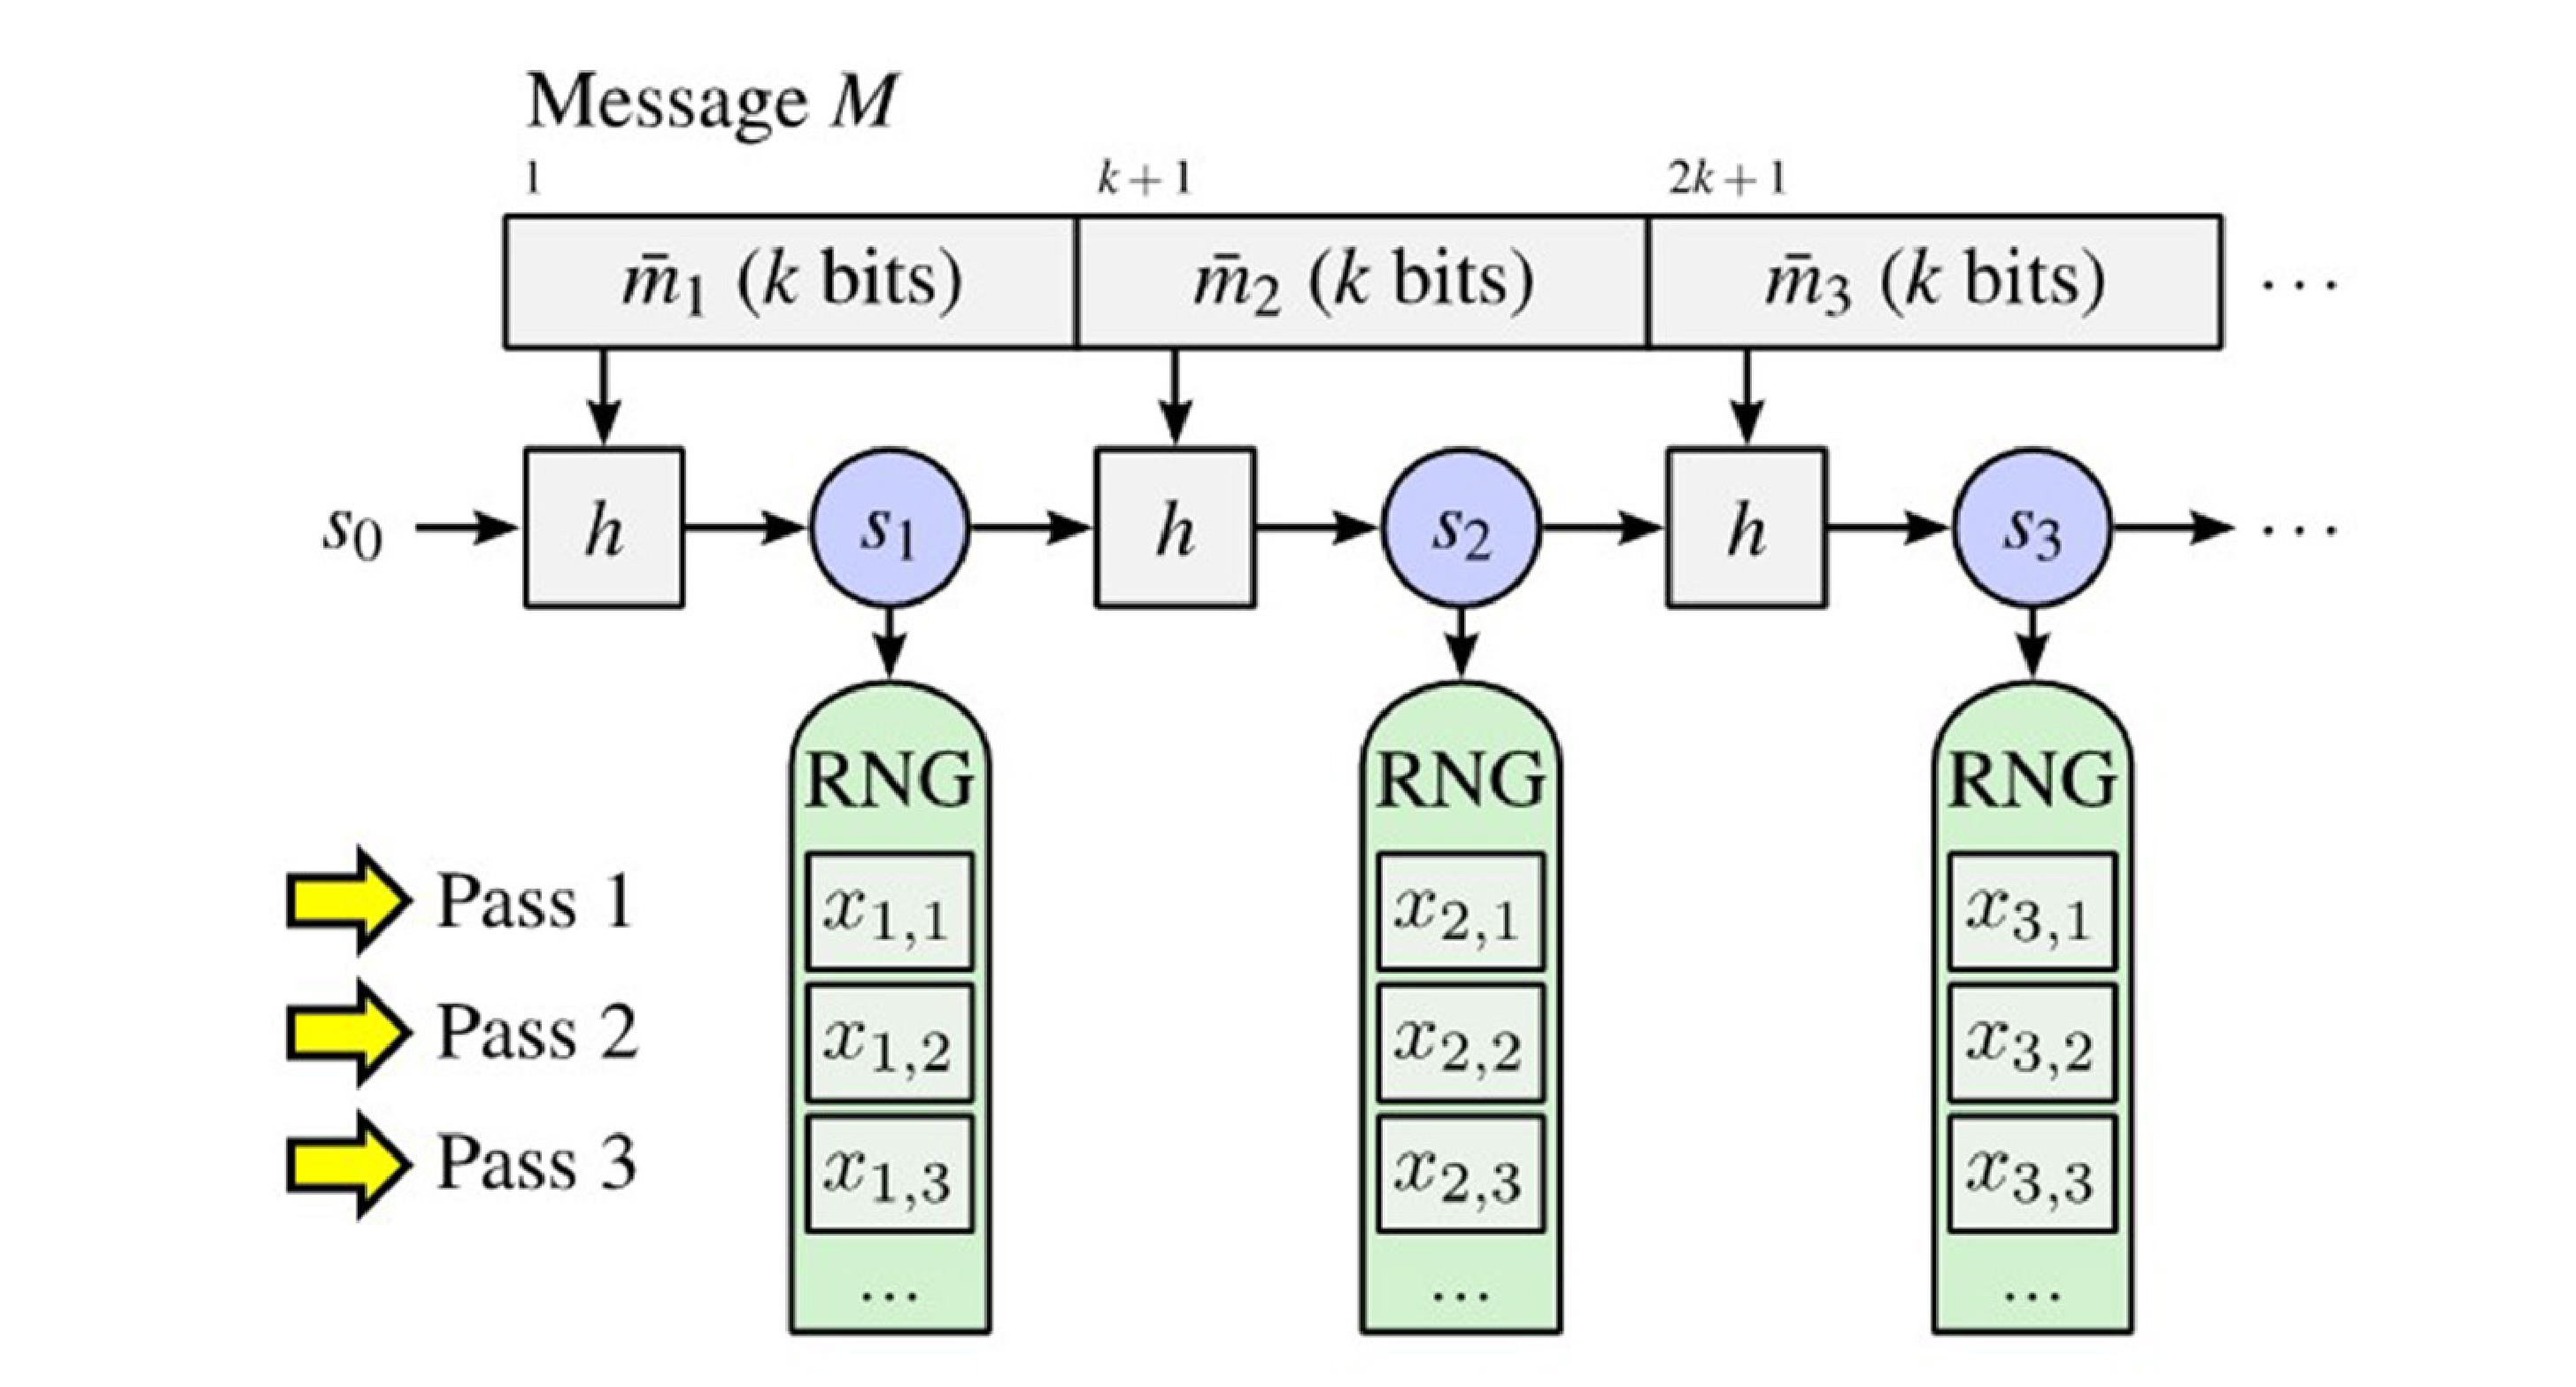
\includegraphics[width=0.9\linewidth]{diagram1.eps}
\end{figure}
\end{frame}

%----------------------------------------------------------

\begin{frame}
\frametitle{Original Diagram}
\begin{figure}
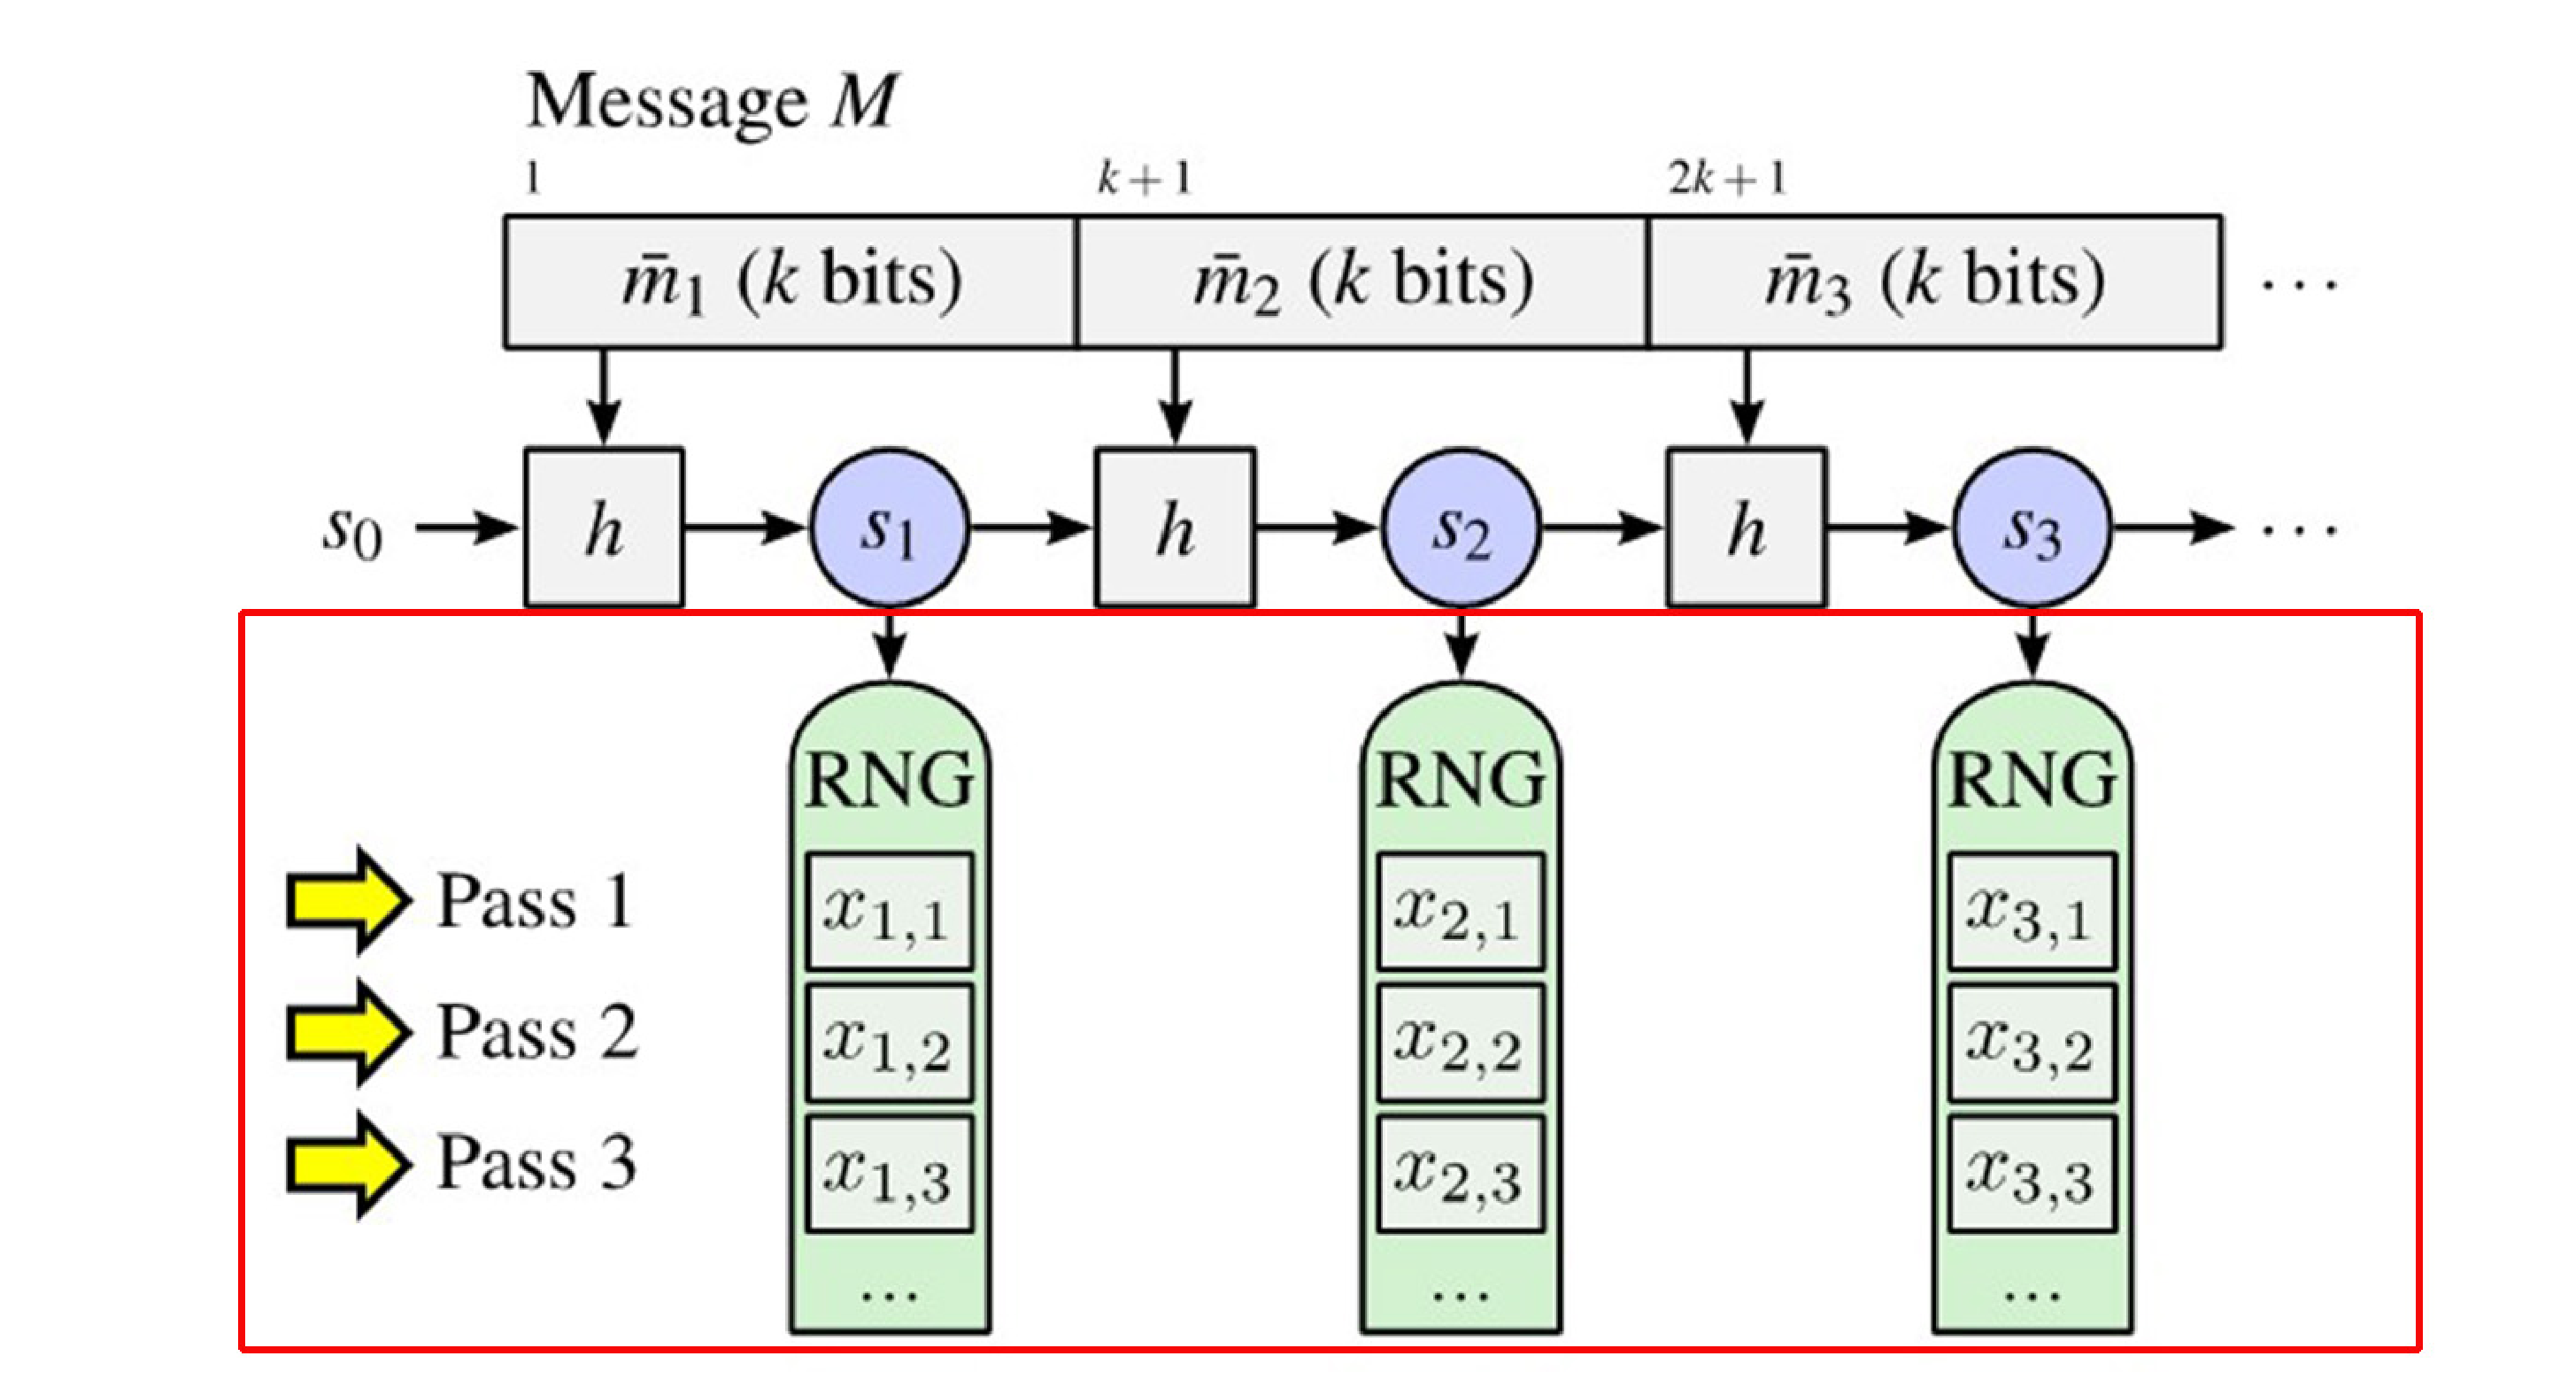
\includegraphics[width=0.9\linewidth]{diagram1_1.eps}
\end{figure}
\end{frame}

%----------------------------------------------------------
\begin{frame}
\frametitle{Modified Diagram}
\begin{figure}
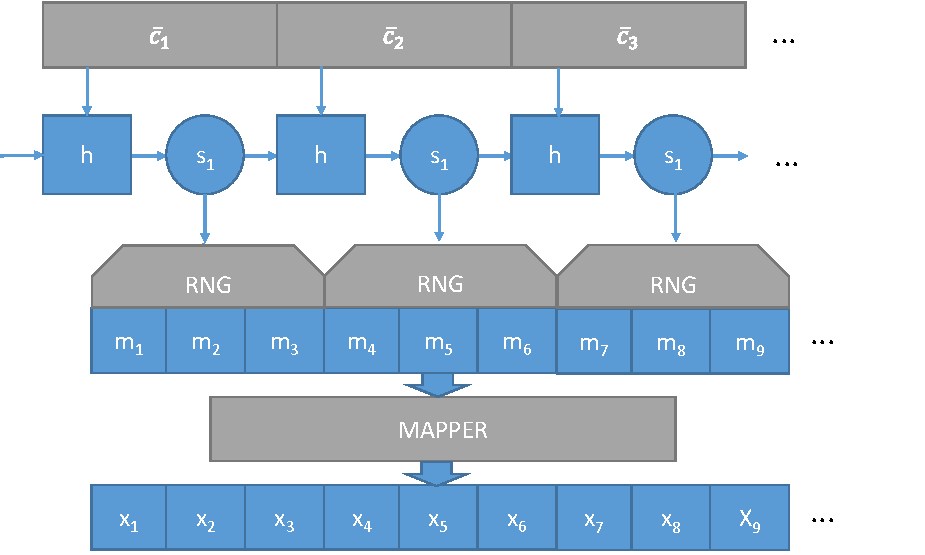
\includegraphics[width=0.8\linewidth]{figencode.pdf}
\end{figure}
\end{frame}

%--------------------------------

\begin{frame}

\frametitle{Simulation Results 2}

\begin{columns}[c]
\column{.7\textwidth}
\begin{figure}
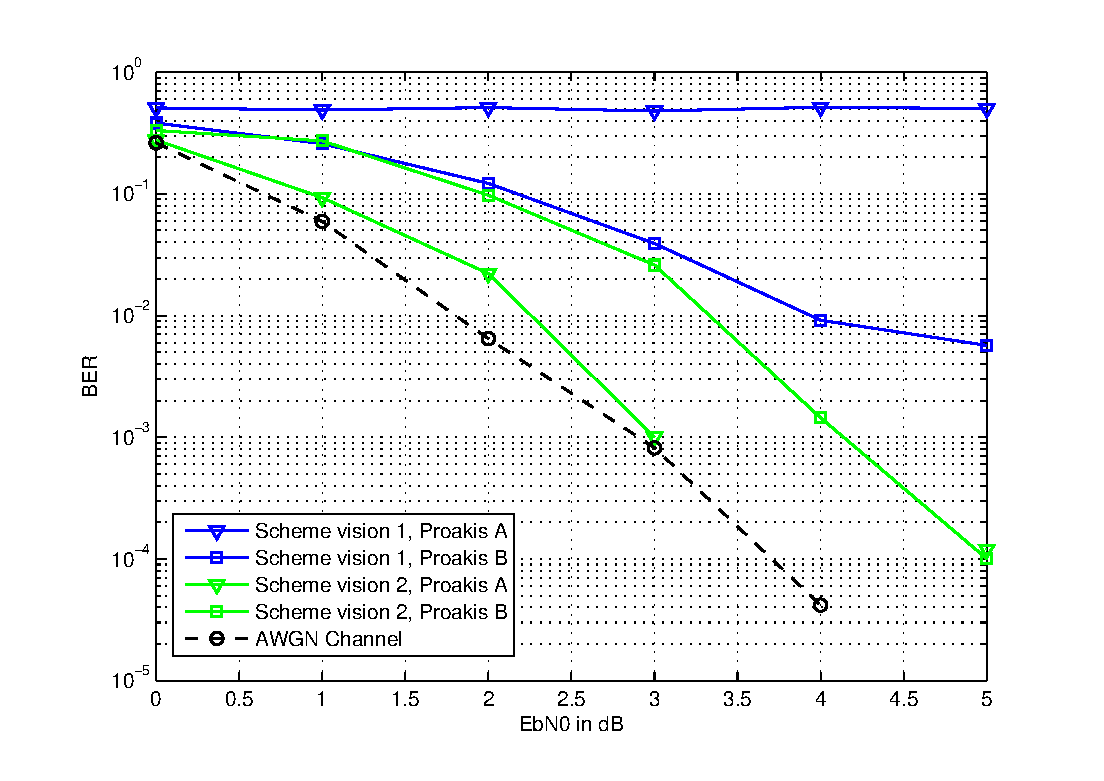
\includegraphics[width=.99\textwidth]{figure_vision2.eps}
\end{figure}

\column{.3\textwidth}
\end{columns}

\end{frame}

%*******************************************************

\subsection{Modification of I/Q Paths}
\begin{frame}
\frametitle{Modification of I/Q Paths}
After the modification before. If the group length is long enough the only correlation just exits between adjacent spines. To break these correlations make the adjacent spines are sent respectively by I/Q paths.
\begin{figure}
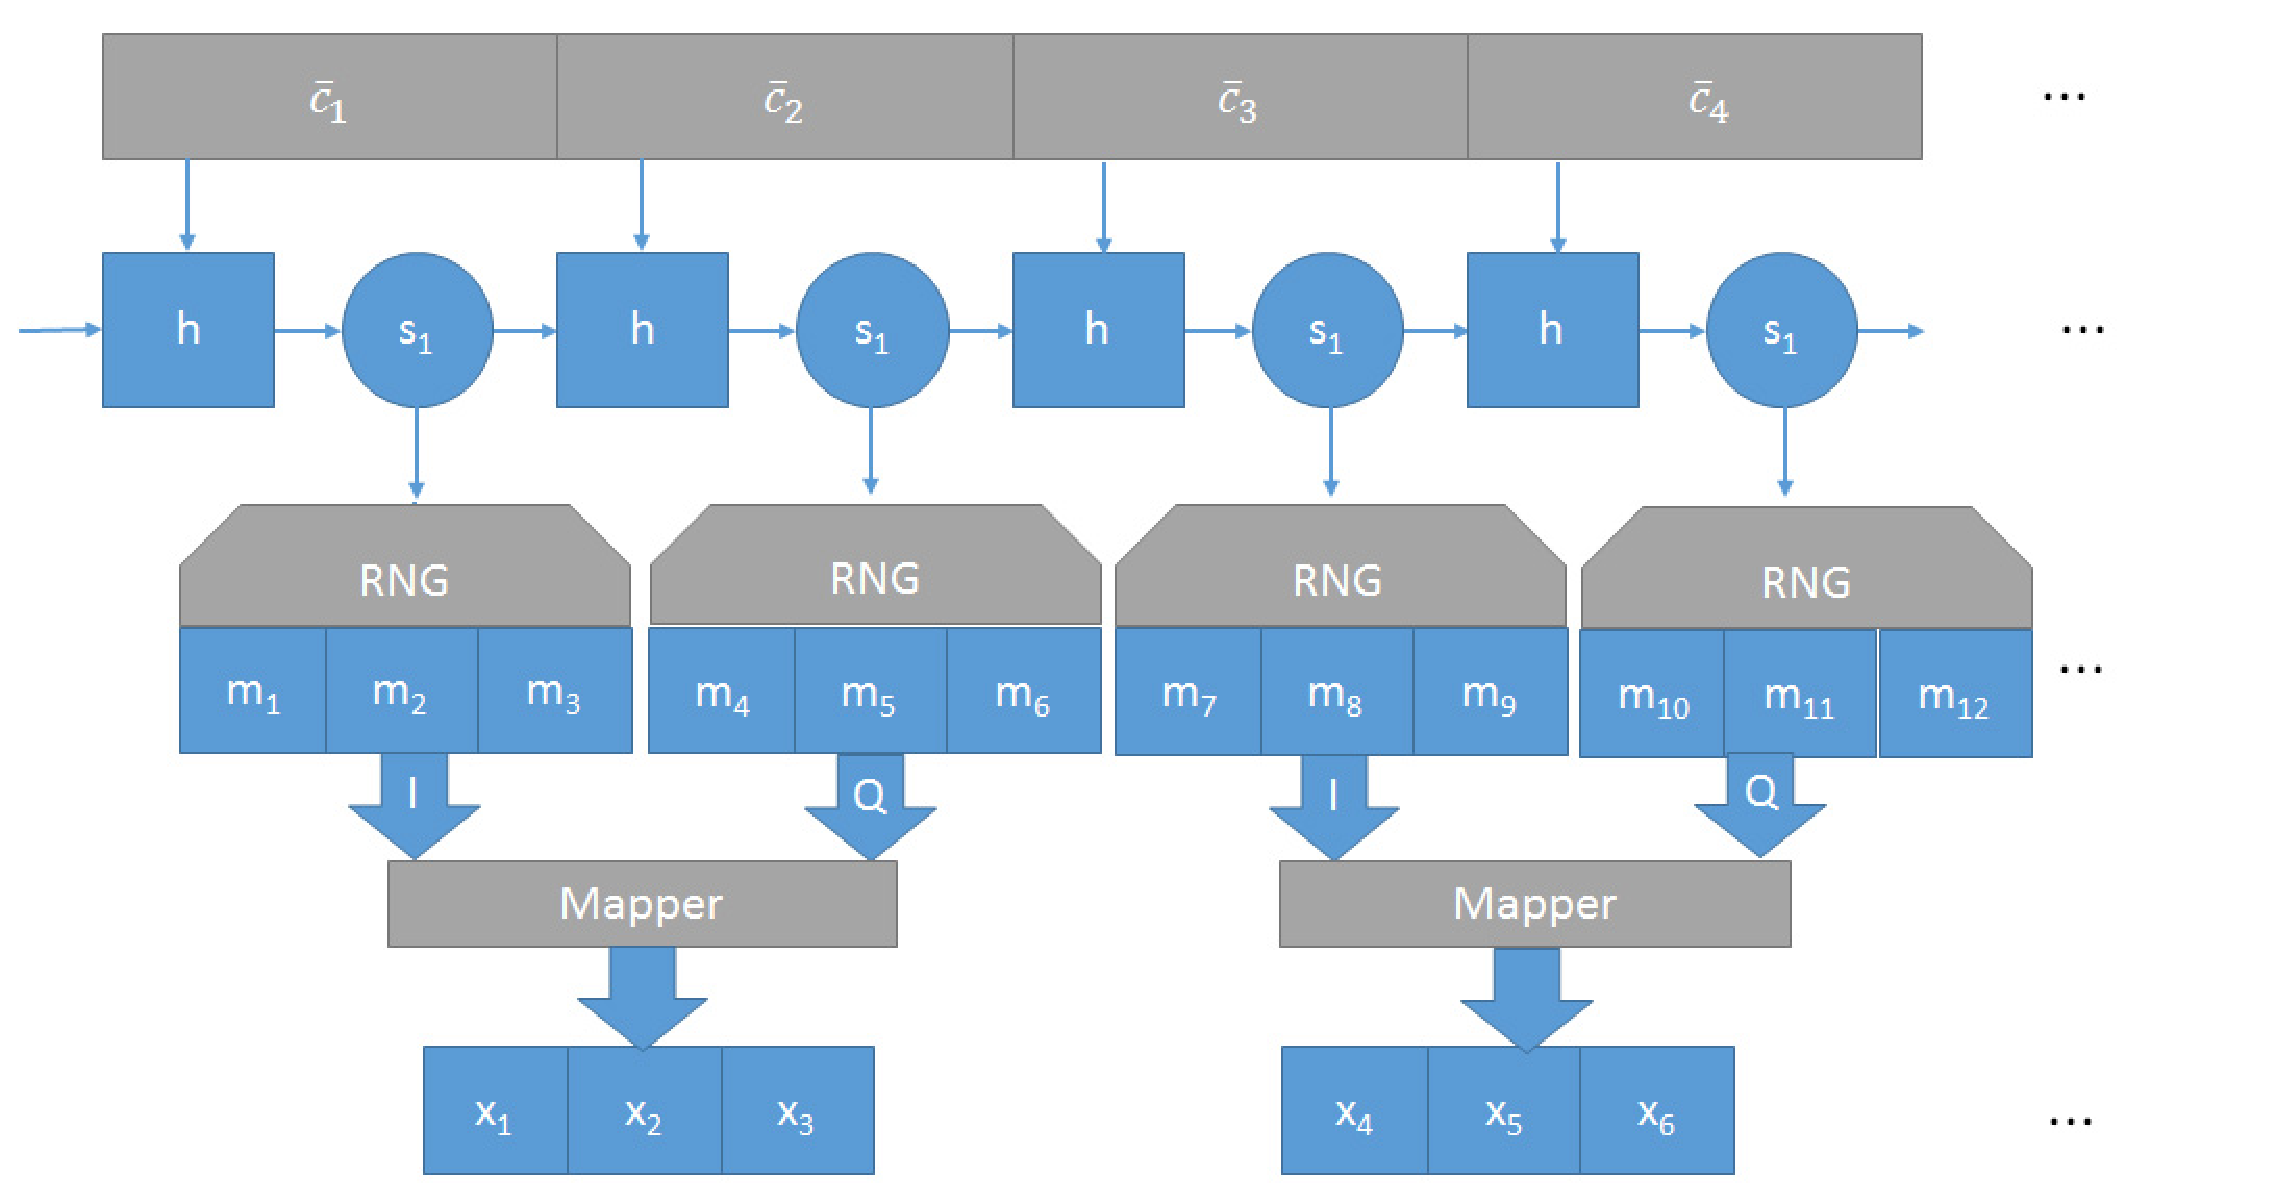
\includegraphics[width=0.8\linewidth]{diagram_v3.eps}
\end{figure}
\end{frame}

%-------------------------------------------------------

\begin{frame}
\frametitle{Simulation Results 1}
\begin{columns}[c]
\column{.7\textwidth}
\begin{figure}
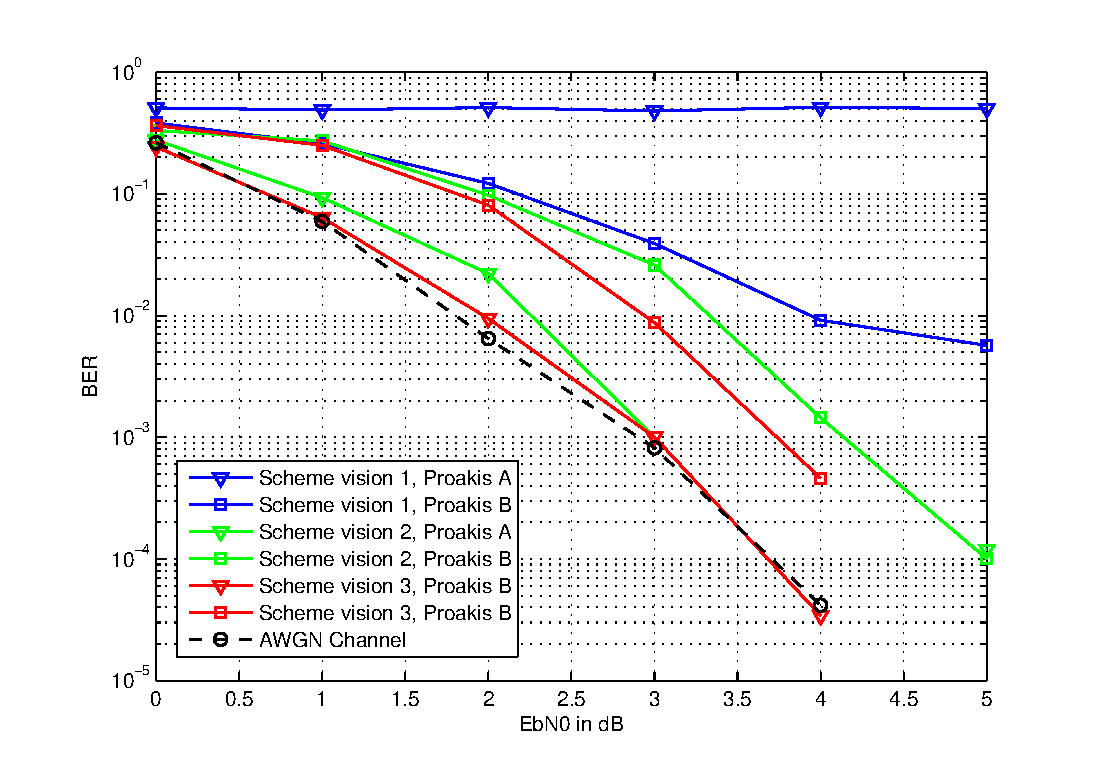
\includegraphics[width=.99\textwidth]{figure_vision3.eps}%wait for figure
\end{figure}
\column{.3\textwidth}
After the modification the results of channel Proakis A have been very closed to the AWGN performance. But the Proakis B one is still high. 
\end{columns}

\end{frame}
%------------------------------------------------
\end{document} 
